\section{Experimental Uncertainties}\label{sec-unc}
Several types of experimental uncertainties need to be taken into account for the combind analysis, to cover systematics effect due to the detector performance, the reconstruction of objects such as leptons and jets, and the effects of flavour tagging. Table \ref{tab:ExpSysts} summarises these various contributions that are sources of uncertainty.

\begin{table}
    \centering
    \renewcommand{\arraystretch}{1.2}
    \resizebox{1.05\textwidth}{!}{%
      \begin{tabular}{llr}
        \hline \hline
        \textbf{Systematic uncertainty name} & $\quad\quad\quad\quad\quad$ \textbf{Description} &\textbf{Regime} \\
        \hline
        \multicolumn{3}{c}{Luminosity and Pile-up}\\
        \hline
        \texttt{LUMI\_2015\_2018 }& Uncertainty on total integrated luminosity & All \\
        \texttt{PRW\_DATASF}& Uncertainty on pile-up modelling & All \\
        \hline
        \multicolumn{3}{c}{\etm and $E_{\text{T,trk}}^{\text{miss}}$}\\
        \hline
        \texttt{MET\_SoftTrk\_ResoPara(Perp)}&  Soft term longitudinal (transverse) resolution uncertainty & All \\
        \texttt{MET\_SoftTrk\_Scale   }&  Soft term scale uncertainty & All \\
        \texttt{MET\_JetTrk\_Scale    }& $E_{\text{T,trk}}^{\text{miss}}$ scale uncertainty & All \\
        \texttt{METTrig\{Stat,Top,Z,Sumpt\}} & Trigger efficiency uncertainty & Resolved \\
        \hline
        \multicolumn{3}{c}{Electrons}\\
        \hline
        \texttt{EL\_EFF\_Trigger\_TOTAL}&  Trigger efficiency uncertainty & All \\
        \texttt{EL\_EFF\_Reco\_TOTAL}&  Reconstruction efficiency uncertainty & All \\
        \texttt{EL\_EFF\_ID\_TOTAL}&  Identification (ID) efficiency uncertainty & All \\
        \texttt{EL\_EFF\_Iso\_TOTAL}&  Isolation efficiency uncertainty & All \\
        \texttt{EG\_SCALE\_ALL}&        Energy scale uncertainty   &  all  \\
        \texttt{EG\_RESOLUTION\_ALL}&    Energy resolution uncertainty  & All \\
        \hline
        \multicolumn{3}{c}{Muons}\\
        \hline
        \texttt{MUON\_EFF\_RECO\_\{STAT,SYS\} }& {Reconstruction and ID efficiency uncertainty for muons with $p_T > 15$ GeV} & All \\
        \texttt{MUON\_EFF\_RECO\_\{STAT,SYS\}\_LOWPT }&{Reconstruction and ID efficiency uncertainty for muons with $p_T \leq 15$ GeV} & All \\
        \texttt{MUON\_EFF\_ISO\_\{STAT,SYS\} }& {Isolation efficiency uncertainty} & All \\
        \texttt{MUON\_EFF\_TTVA\_\{STAT,SYS\} }& {Track-to-vertex association efficiency uncertainty} & All \\
        \texttt{MUON\_SCALE}&    Momentum scale uncertainty & All \\
        \texttt{MUON\_SAGITTA\_RHO(RESBIAS)} & Momentum scale uncertainty to cover charge-dependent local misalignment effects & All \\
        \texttt{MUON\_ID(MS) }& Momentum resolution uncertainty of the inner detector (muon spectrometer) & All \\
        \texttt{MUON\_EFF\_Trig\{Stat,Sys\}Uncertainty} & Trigger efficiency uncertainty & All \\
        \hline
        \multicolumn{3}{c}{Taus}\\
        \hline
        \texttt{TAUS\_TRUEHADTAU\_EFF\_RECO\_TOTAL}& {Reconstruction efficiency} & All \\
        \texttt{TAUS\_TRUEHADTAU\_EFF\_RNNID\_*}& {RNN ID efficiency} & All \\
        \texttt{TAUS\_TRUEHADTAU\_SME\_TES\_*}& {In-Situ tau energy scale correction} & All \\
        \texttt{TAUS\_TRUEELECTRON\_EFF\_ELEBDT\_*}& {Electron Veto efficiency SF} & All \\
        \hline
        \multicolumn{3}{c}{Small-R jets}\\
        \hline
        \texttt{JET\_CR\_BJES\_Response }& Energy scale uncertainties for $b$-jets & All \\
        \texttt{JET\_CR\_EffectiveNP\_Detector\{1-2\} }& Energy scale uncertainties due to in-situ calibration & All \\
        \texttt{JET\_CR\_EffectiveNP\_Mixed\{1-3\} }& Energy scale uncertainties due to in-situ calibration & All  \\
        \texttt{JET\_CR\_EffectiveNP\_Modelling\{1-4\} }& Energy scale uncertainties due to in-situ calibration & All \\
        \texttt{JET\_CR\_EffectiveNP\_Statistical\{1-6\} }& Energy scale uncertainties due to in-situ calibration & All \\
        \texttt{JET\_CR\_EtaIntercal\_Modelling}& Energy scale uncertainties to cover $\eta$-intercalibration non-closure & All \\
        \texttt{JET\_CR\_EtaIntercal\_NonClosure\_highE}& Energy scale uncertainties to cover $\eta$-intercalibration non-closure & All \\
        \texttt{JET\_CR\_EtaIntercal\_NonClosure\_negEta}& Energy scale uncertainties to cover $\eta$-intercalibration non-closure & All \\
        \texttt{JET\_CR\_EtaIntercal\_NonClosure\_posEta}& Energy scale uncertainties to cover $\eta$-intercalibration non-closure & All \\
        \texttt{JET\_CR\_EtaIntercal\_TotalStat}& Energy scale uncertainties to cover $\eta$-intercalibration non-closure & All \\
        \texttt{JET\_CR\_Flav\_Comp(Flavor\_Response) }& Energy scale uncertainty related to flavour composition (response) & All \\
        \texttt{JET\_CR\_PunchTroughMC16 }& Energy scale uncertainty for 'punch-through' & All \\
        \texttt{JET\_CR\_SingleParticle\_HighPt }& Energy scale uncertainty for the behavior of high-\pt\ single hadrons & All \\
        \texttt{JET\_CR\_JER\_DataVsMC}& Energy resolution total uncertainty  & All \\
        \texttt{JET\_CR\_JER\_EffectiveNP\_\{1-6,7restTerm\}}& Energy resolution total uncertainties & All \\
        \texttt{JET\_JvtEfficiency}& JVT efficiency uncertainty  & All \\
        \texttt{JET\_PU\_\{OffsetMu(NPV),PtTerm,RhoTopology\}}& Energy scale uncertainties due to pile-up effects & All \\
        \hline
        \multicolumn{3}{c}{Large-R jets}\\
        \hline
        \texttt{FJ\_JMSJES\_Baseline\_Kin }&  {Energy and mass scale uncertainty due to basic data-simulation differences} & Boosted \\
        \texttt{FJ\_JMSJES\_Modelling\_Kin }& {Energy and mass scale uncertainty due to simulation differences} & Boosted \\
        \texttt{FJ\_JMSJES\_Tracking\_Kin }&  {Energy and mass scale uncertainty on reference tracks} & Boosted \\
        \texttt{FJ\_JMSJES\_TotalStat\_Kin }& {Energy and mass scale uncertainty from stat. unc. on the measurement} & Boosted \\
        \texttt{FJ\_JER }&  Energy resolution uncertainty & Boosted \\
        \texttt{FJ\_JMR }&  Mass resolution uncertainty & Boosted \\
        \hline
        \multicolumn{3}{c}{Flavour tagging: PFlow jets }\\
        \hline
        \texttt{FT\_EFF\_PFlow\_Eigen\_B\_\{0-44\}}& {Tagging efficiency uncertainties for $b$-jets} & Resolved \\
        \texttt{FT\_EFF\_PFlow\_Eigen\_C\_\{0-19\}}&{Tagging efficiency uncertainties for $c$-jets} & Resolved \\
        \texttt{FT\_EFF\_PFlow\_Eigen\_Light\_\{0-19\}}&{Tagging efficiency uncertainties for light-jets} & Resolved \\
        \texttt{FT\_EFF\_PFlow\_extrapolation }& Tagging efficiency uncertainty for high-\pt\ jets & Resolved \\
        \hline
        \multicolumn{3}{c}{$b$-tagging: VR track jets}\\
        \hline
        \texttt{FT\_EFF\_VR\_Eigen\_B\_\{0-4\}}& {$b$-tagging efficiency uncertainties for $b$-jets} & Boosted \\
        \texttt{FT\_EFF\_VR\_Eigen\_C\_\{0-3\}}&{$b$-tagging efficiency uncertainties for $c$-jets} & Boosted \\
        \texttt{FT\_EFF\_VR\_Eigen\_Light\_\{0-3\}}&{$b$-tagging efficiency uncertainties for light-jets} & Boosted \\
        \texttt{FT\_EFF\_VR\_extrapolation }& $b$-tagging efficiency uncertainty for high-\pt\ jets & Boosted \\
        \hline \hline
    \end{tabular}
    }
    \caption{Summary of all experimental systematic uncertainties. }
    \label{tab:ExpSysts}
    \renewcommand{\arraystretch}{1.0}
  \end{table}
   %TODO check that the ftag uncertainties are still completely decorrelated for the VR track and PFlow

\paragraph{Luminosity \& Pile-up:} The measured Run 2 luminosity for ATLAS is 140 fb$^{-1}$ with an uncertainty of 0.83\% \cite{ATLAS:2022hro}. The measurement is performed with $x-y$ beam separation scans combined with information from dedicated lumonisity-sensitive detectors. The pile-up uncertainty for simulated events is obtained by varying the data rescaling factor of the nominal average pile-up $\langle \mu \rangle$. \gls{mc}-simulated samples match data at a higher $\mu$, so this rescaling factor is used to reweight the data, matching a simulated $\mu = 1.0$ to a data-$\mu = 1.09$, written $1.0/1.09$. The 1$\sigma$ uncertainty is measured by varying the factor from $1.0/1.0$ to $1.0/1.18$. % TODO check this is still true: comes from Maria's thesis.

\paragraph{Triggers} Uncertainties on the trigger efficiencies are derived for the electron, muon, and \etm triggers. The electron trigger uncertainty combines the statistical and systematic effect, while for the muon triggers they are considered seperately. Scale factors to the \etm trigger efficiency are derived on $W+$jets events, taking into acount the statistics of the dataset, assessing systematic effects by deriving the \gls{sf}s with alternative top and $Z$+jets samples, and a final uncertainty modelling the efficiency dependency on the scalar sum of all final state jets. % TODO too close to Maria.

\paragraph{Leptons \& \etm\ Reconstruction} Leptons and \etm\ reconstructions were calibrated in dedicated analyses. A reduced set of uncertainties are propagated to the combined \vhbc, and include:
\begin{itemize}
    \item \etm: \gls{sf}s factors are included to account for the direction of the \etm\ as well as the soft term contributions. % TODO link to etm in detector 
    \item Electrons: uncertainties on the reconstructed values, the identification efficiency, isolation efficiency and the energy scale and resolution are included. These are derived by comparing data and simulations kinematic distributions in a $Z \rightarrow e^+ e^-$, $W\rightarrow e\nu$, and $J/\psi \rightarrow e^+e^-$ events \Cite{Aaboud:2657964}. 
    \item Muons: uncertaintes on the reconstruction and identification efficiencies for muons with $p_T > 15$ GeV and $p_T < 15$ are included separately, using respectively samples of $Z\rightarrow \mu^+\mu^-$ and $J/\psi \rightarrow \mu^+\mu^-$ \cite{Aad:2746302}. Additional, uncertainties on the isolation efficiency, track-to-vertex association efficiency, momentum scale and resolution as well as charge-dependent misalignement effects are considered. 
    \item Taus: hadronically decaying $\tau$-leptons\footnote{About $65$\% of $\tau$ decays are hadronic.} uncertainties on the reconstruction and \gls{rnn}-based identification efficiencies as well as the electron veto efficiencies are derived from samples of $Z\rightarrow\tau^+ \tau^-$ and top-quark decays to taus \cite{ATL-PHYS-PUB-2019-033, ATL-PHYS-PUB-2015-045, ATLAS-CONF-2017-029}.
\end{itemize}

\paragraph{Jets} Jets are calibrated in dedicated analyses, of which two reduced sets of uncertainties are propagated to the combined \vhbc for small- and large-$R$ jets. For the small-$R$ jets, these uncertainties cover \textit{in-situ} analyses, $\eta$-intercalibration, flavour composition, punch-through jets, high-$p_T$ hadrons, and pile-up effects as well as the jet energy scale and resolution measured in data \cite{ATLASjesjerMeas, Aad:2854733}. The reduced set is derived by a principal component analysis to preserve correlations in certain regions of jet kinematics. Large-$R$ jets uncertainties for the energy scale and resolution are also estimated from data \cite{ATLAS:2018bip}. An uncertainty covering the calibration discrepancy between data and \gls{mc}-simulations is also included.

\paragraph{Flavour Tagging} A dedicated calibration is performed to derive flavour tagging scale factors in the resolved regime, as described in Section \ref{sec-selectionandcat}, while the common ATLAS uncertainties are used for the boosted regime, as described in \ref{chap-calibration}. These flavour tagging calibration \gls{sf}s are derived by combining data-\gls{mc} efficiency modelling \gls{sf}s and \gls{mc}-\gls{mc} \gls{sf}s to account for parton showering and hadronisation variations. These scale factors are smoothed using a local polynomial kernel estimator to avoid distortions in the kinematic variables \cite{ATL-PHYS-PUB-2020-004}. For each jet flavour, there is one uncertainty per $p_T$ bin in the calibration. A principal component analysis is deployed to reduce the large set of systematic uncertainties to 45 (5) for $b$-jet, 20 (4)for $c$-jet, and 20 (4) for light-jets in the resolved (boosted) regime. An extra uncertainty is added to model the effect of high-$p_T$ jets. Truth tagging uncertainties are covered by these flavour tagging uncertainties.

%
\section{Signal \& Background Modelling}\label{sec-mod}
The modelling of the signal and background in the \vhbc\ combined analysis is discussed in this section. The signal and background composition changes depending on the lepton channel and the analysis category, with some signal regions background composition represented in Figure \ref{fig:backCom}. The $V$+jets backgrounds are the dominant ones in the 0-lepton and 2-lepton channels, while the top processes contribute more in the 1-lepton channel and at larger jet multiplicities. Due to flavour tagging, \vhb\ primarily selects the $bb$-component of the background while \vhc\ has more diverse flavour compositions. In summary:
\begin{itemize}
    \item \textbf{0-lepton}: the dominant background is the $Z$+jets with a sizeable $W+$jets component due to large \etm or a miss-identified hadronic $\tau$ and some top backgrounds for the \vhb\ side particularly.
    \item \textbf{1-lepton}: for the \vhb, top processes are dominant while for \vhc\ a sizeable $W+$jets is present as well as the top (the latter particularly at higher jet multiplicities). Thre is a visible diboson contribution as well as some multi-jet.  
    \item \textbf{2-lepton}: the background is mostly $Z+$jets, followed by the diboson and the top process for \vhb\ (constrained from the Top $e\mu$ CR). 
\end{itemize}

\begin{figure}[h!]
    %\hspace{-2cm}
    \centering
    \makebox[\linewidth][c]{%
        \begin{subfigure}[b]{0.38\textwidth}
            \centering
            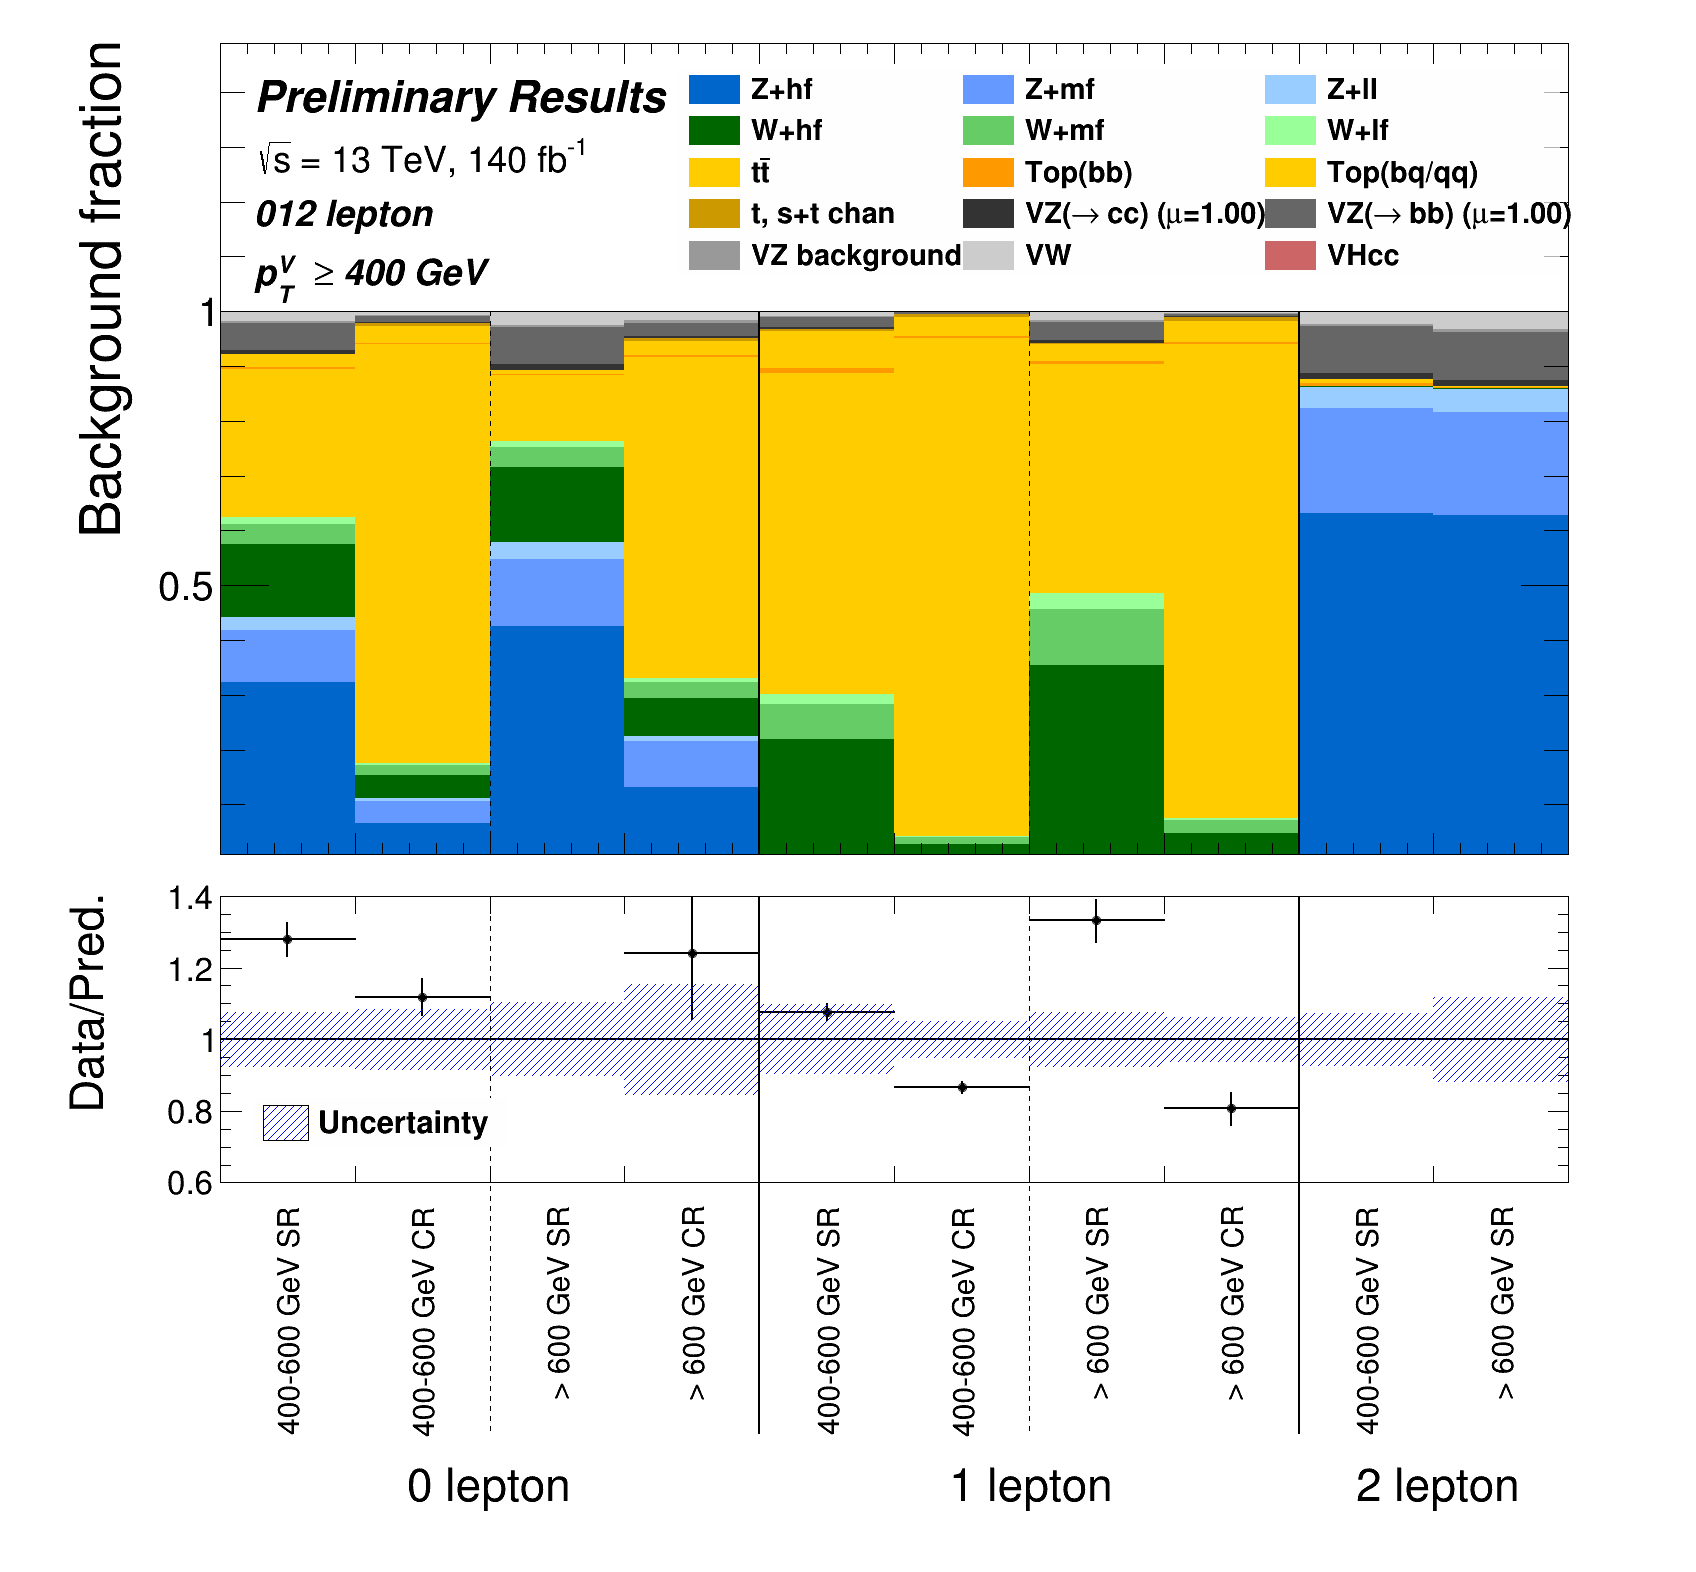
\includegraphics[width=\textwidth]{Images/VH/Own_fit/backCom_uncPrefit/GlobalFit_unconditional__Prefit/C_SRCRs_L012_BMin400.png}
            \caption{Boosted regime.}
            \label{fig:backCom_boos}
        \end{subfigure}
        \begin{subfigure}[b]{0.38\textwidth}
            \centering
            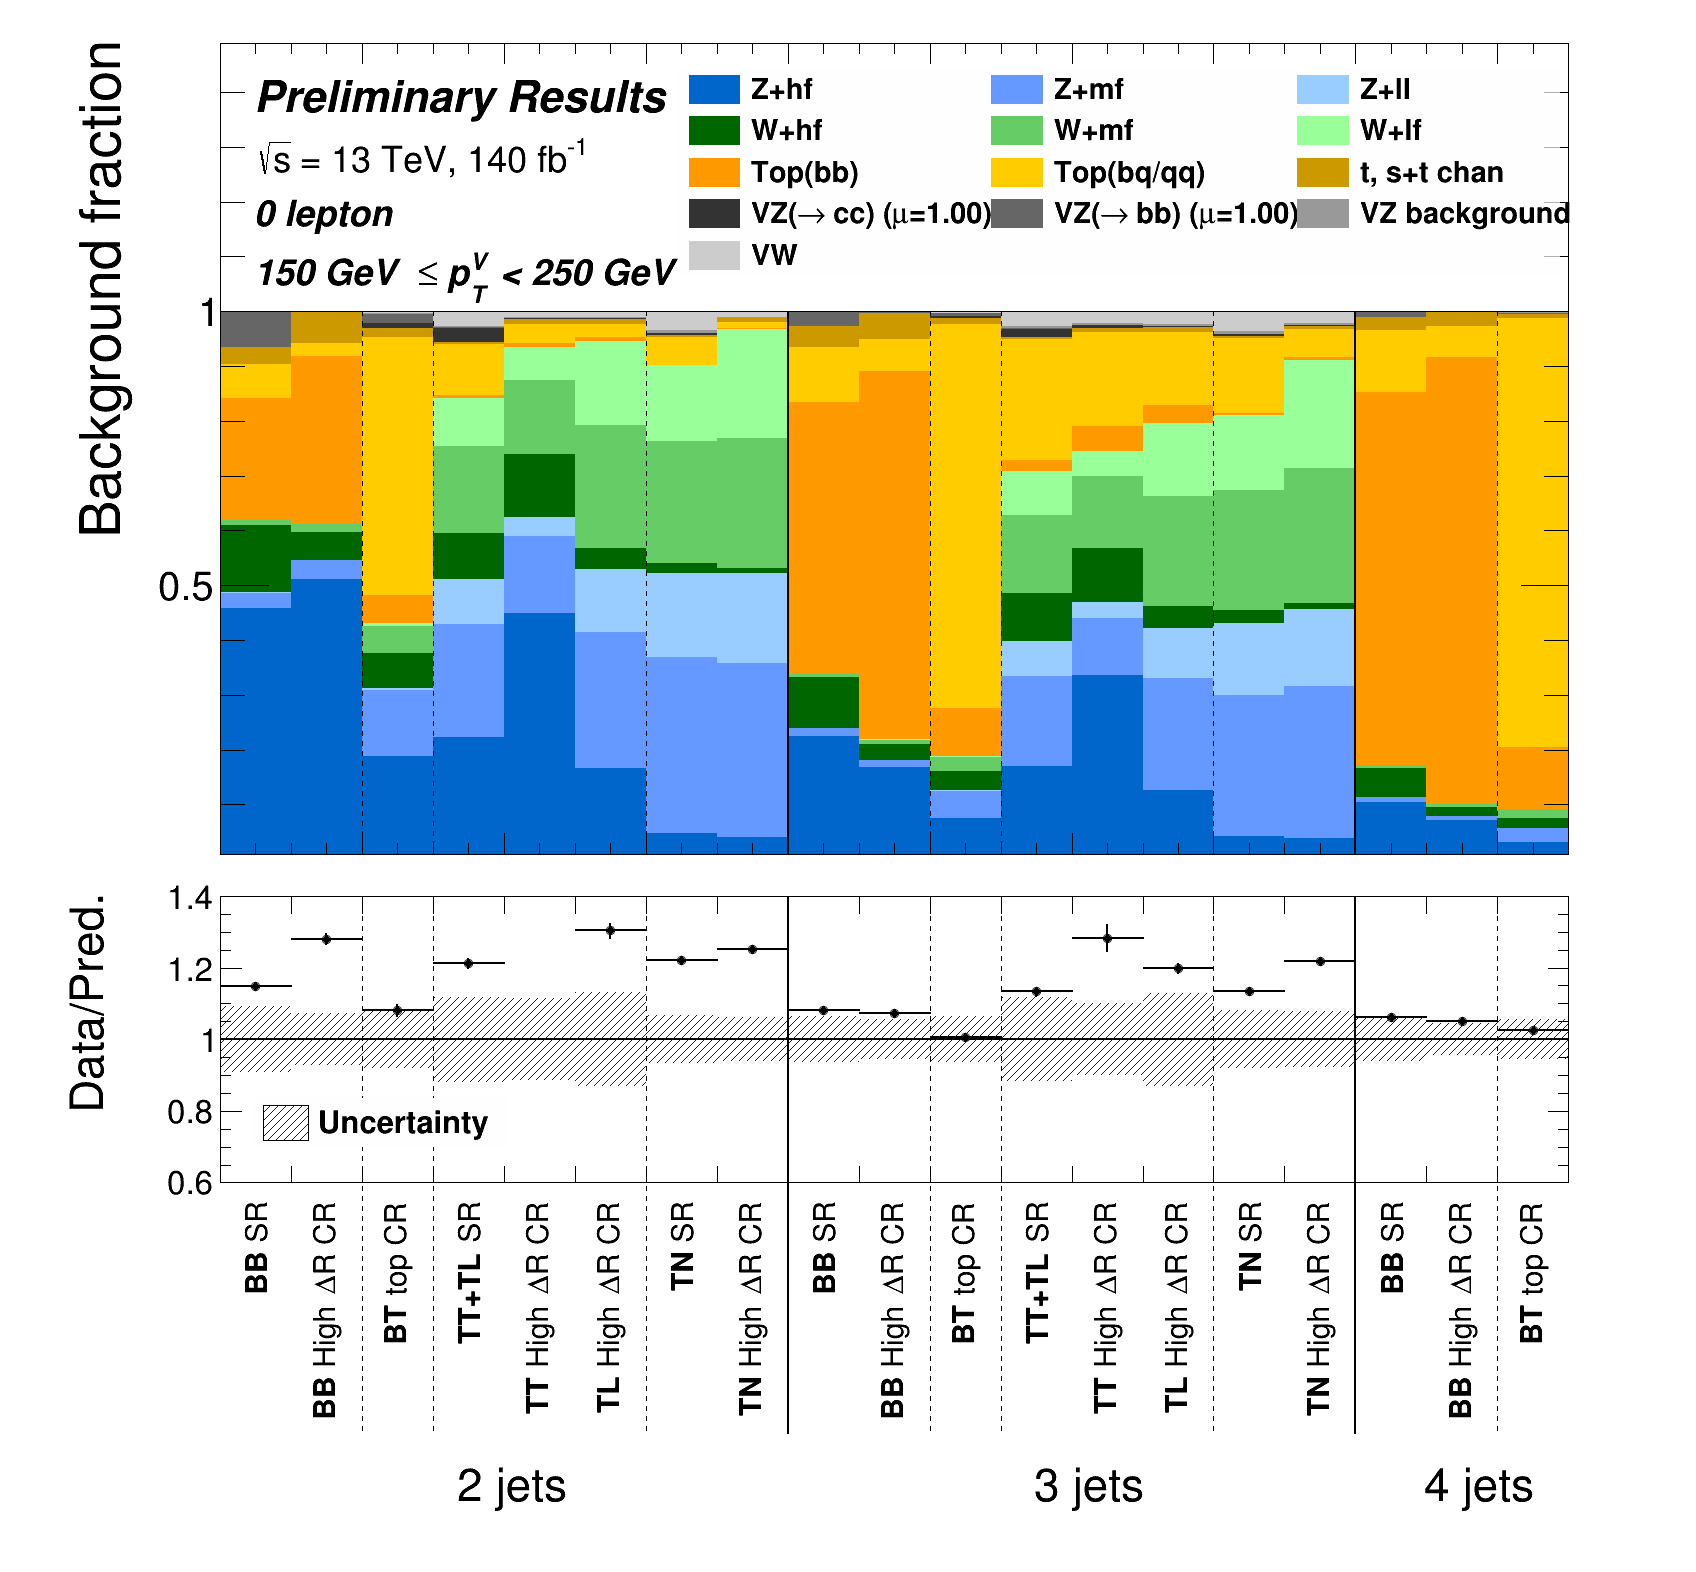
\includegraphics[width=\textwidth]{Images/VH/Own_fit/backCom_uncPrefit/GlobalFit_unconditional__Prefit/C_SRCRs_L0_BMax250_BMin150.png}
            \caption{0L, \ptv\ $\in$ [150, 250] GeV.}
            \label{fig:backCom_0L_1}
        \end{subfigure}
        \begin{subfigure}[b]{0.38\textwidth}
            \centering
            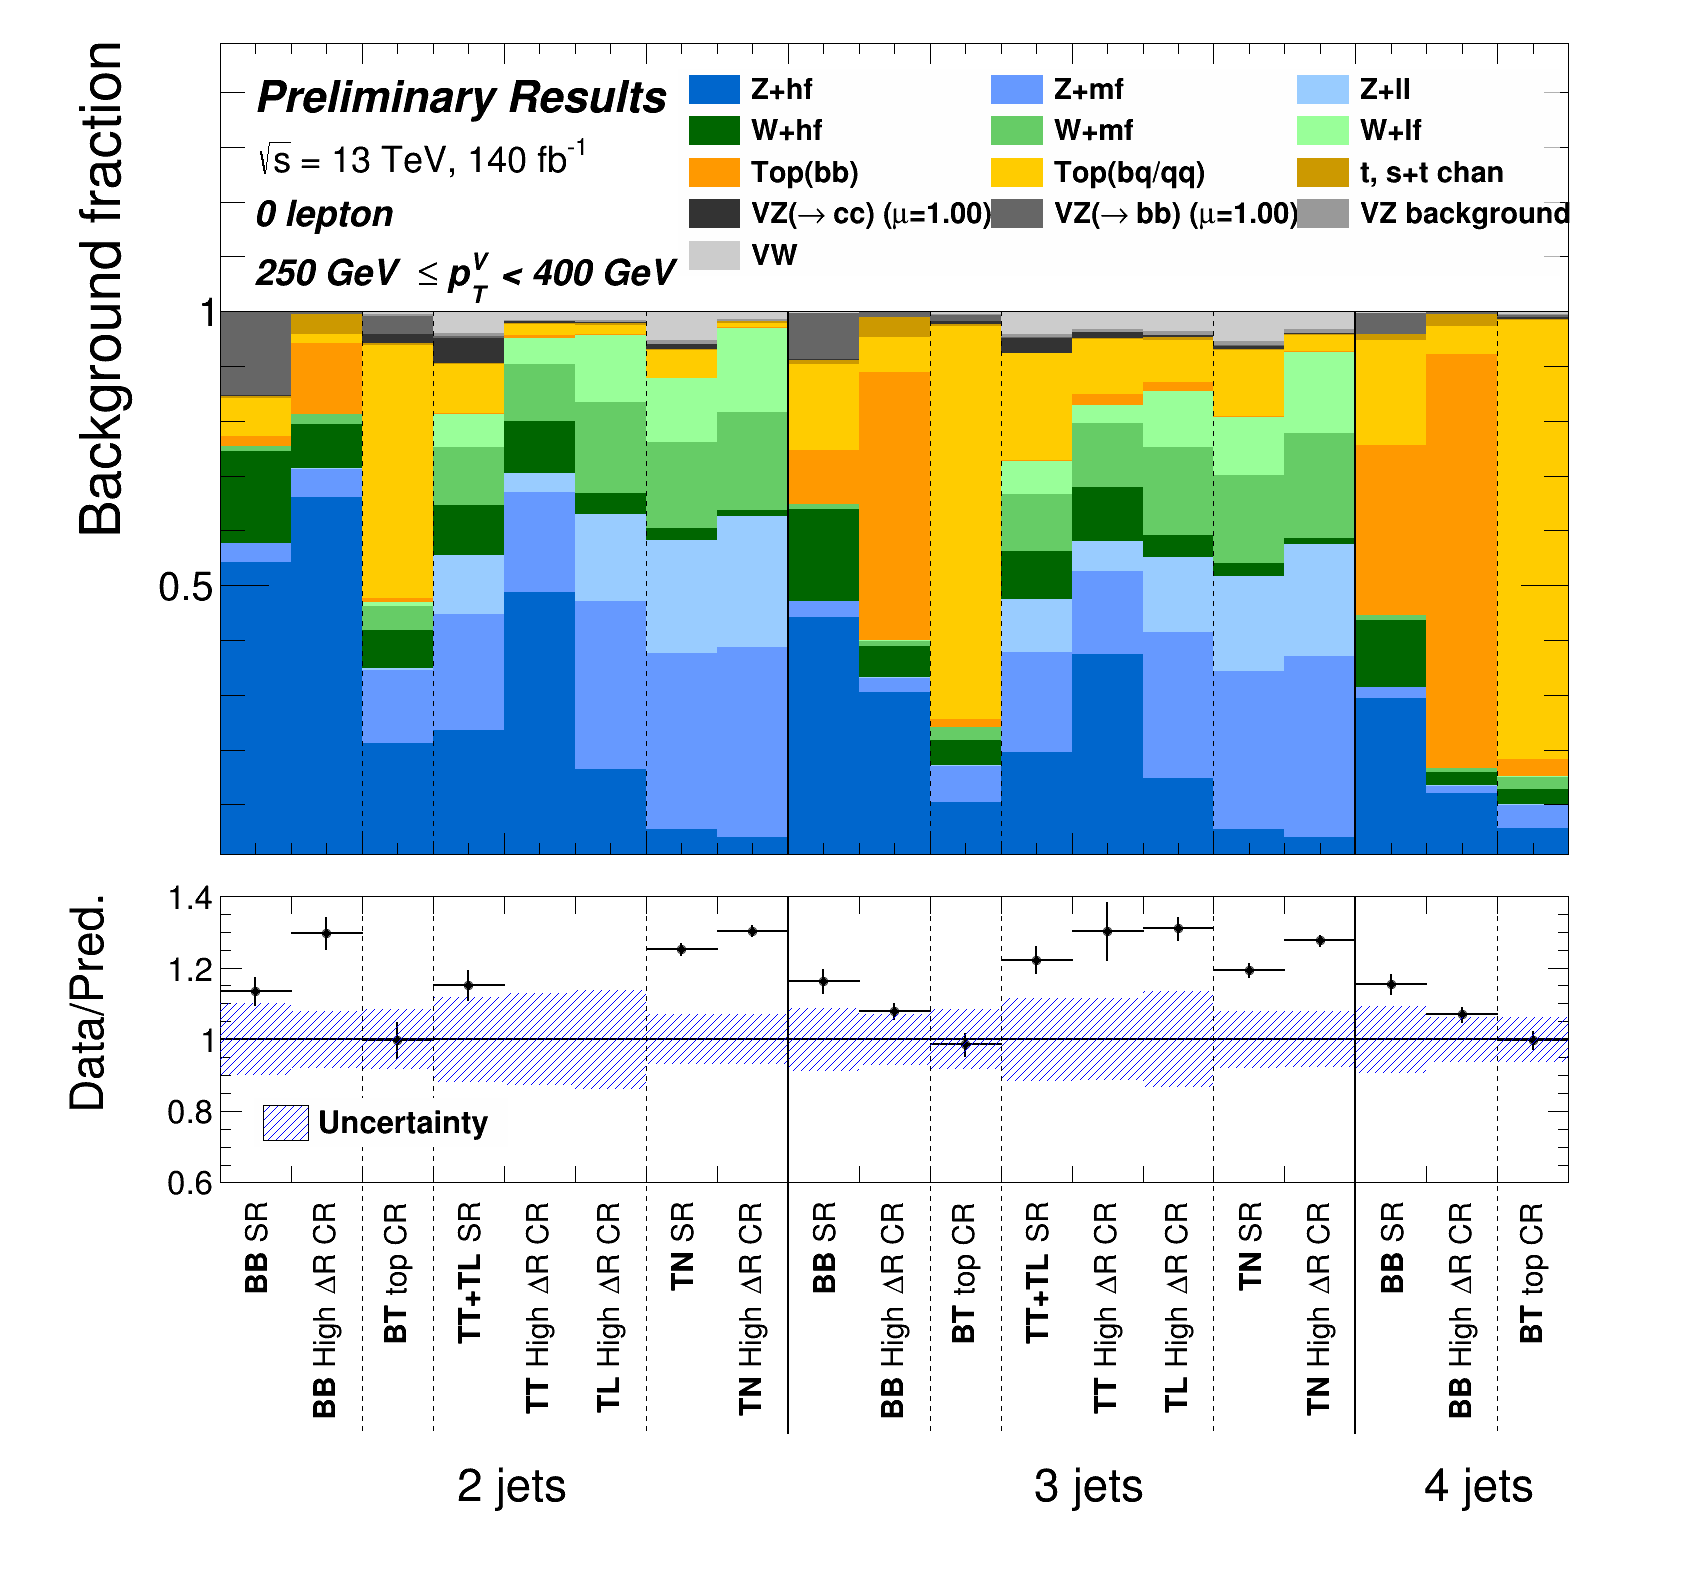
\includegraphics[width=\textwidth]{Images/VH/Own_fit/backCom_uncPrefit/GlobalFit_unconditional__Prefit/C_SRCRs_L0_BMax400_BMin250.png}
            \caption{0L, \ptv\ $\in$ [250, 400] GeV.}
            \label{fig:backCom_0L_2}
        \end{subfigure} 
    }\\
    %\hspace{-2cm}
    \makebox[\linewidth][c]{%
        \begin{subfigure}[b]{0.38\textwidth}
            \centering
            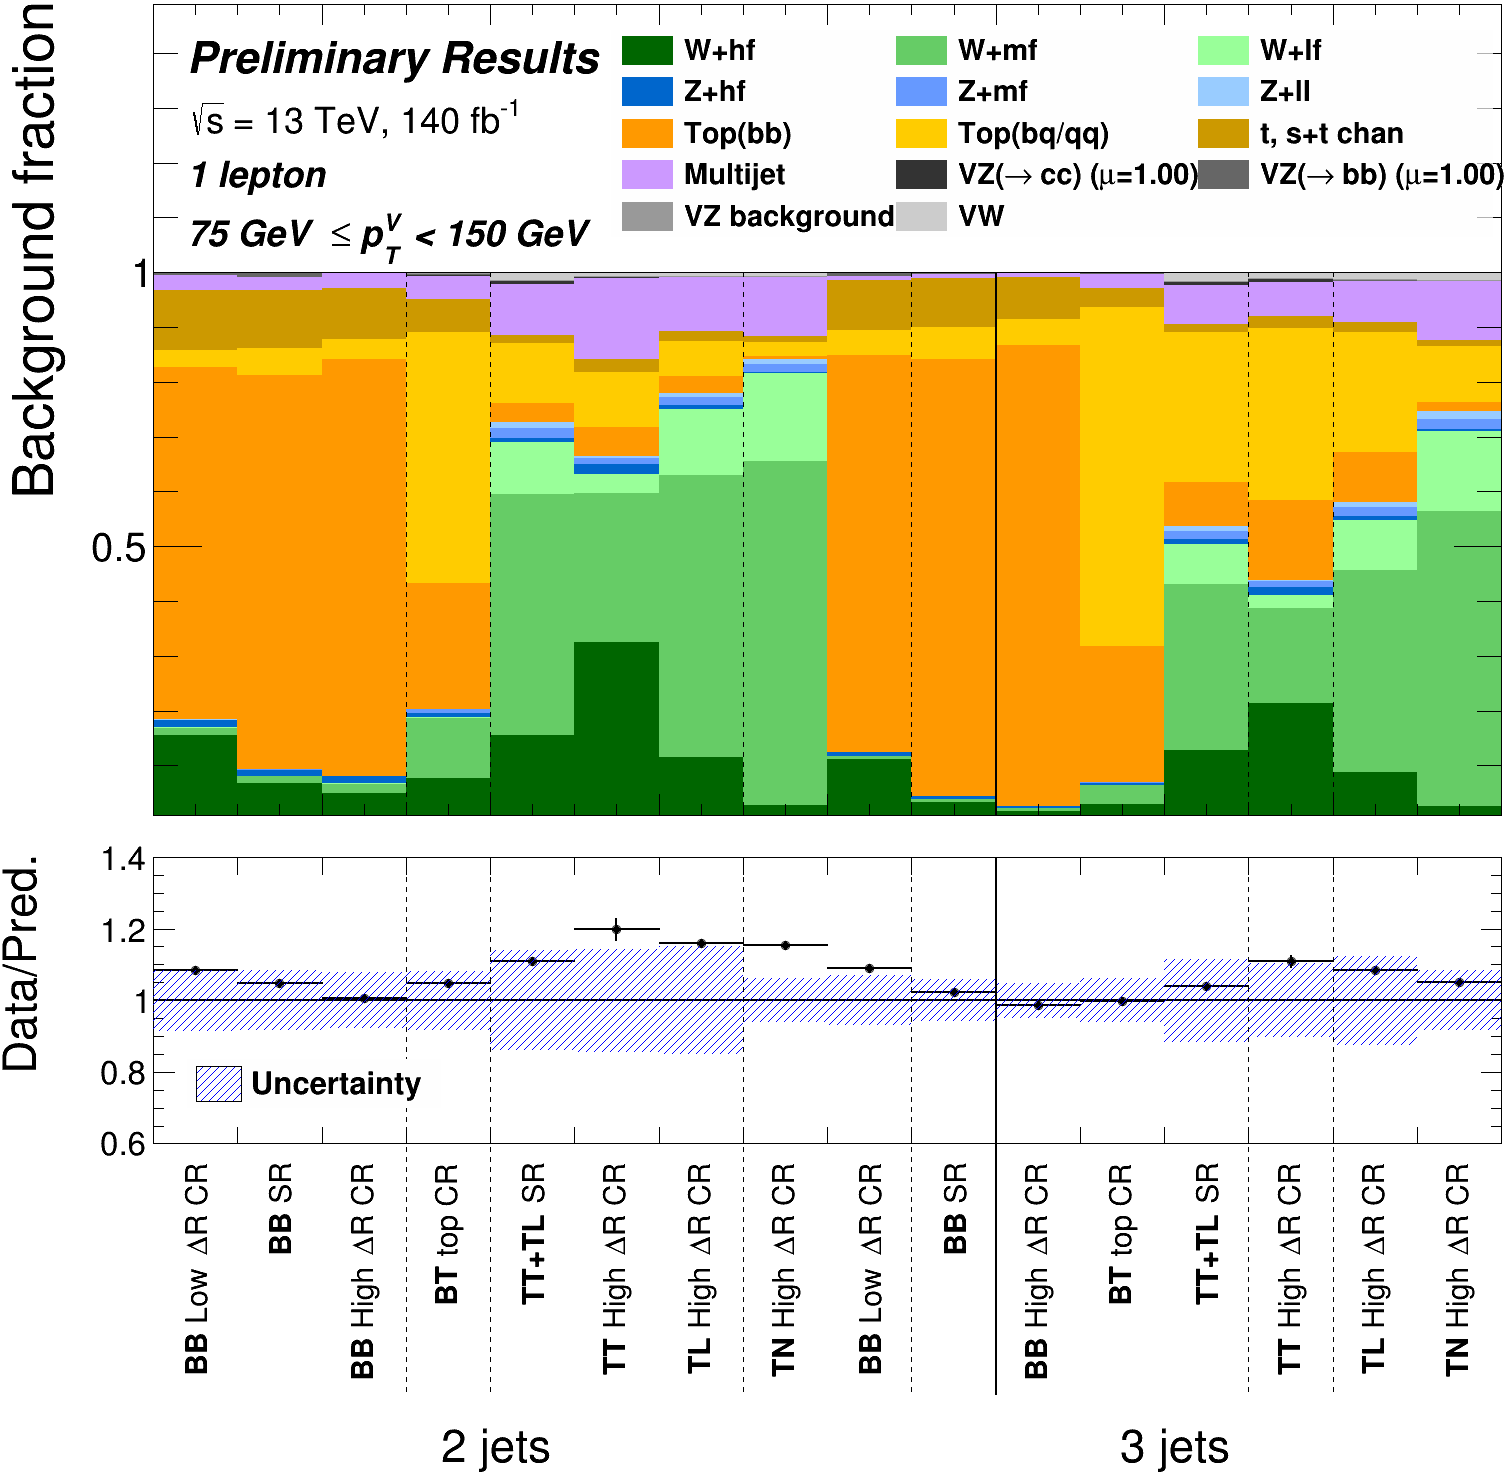
\includegraphics[width=\textwidth]{Images/VH/Own_fit/backCom_uncPrefit/GlobalFit_unconditional__Prefit/C_SRCRs_L1_BMax150_BMin75.png}
            \caption{1L, \ptv\ $\in$ [75, 150] GeV.}
            \label{fig:backCom_1L_1}
        \end{subfigure}
        \begin{subfigure}[b]{0.38\textwidth}
            \centering
            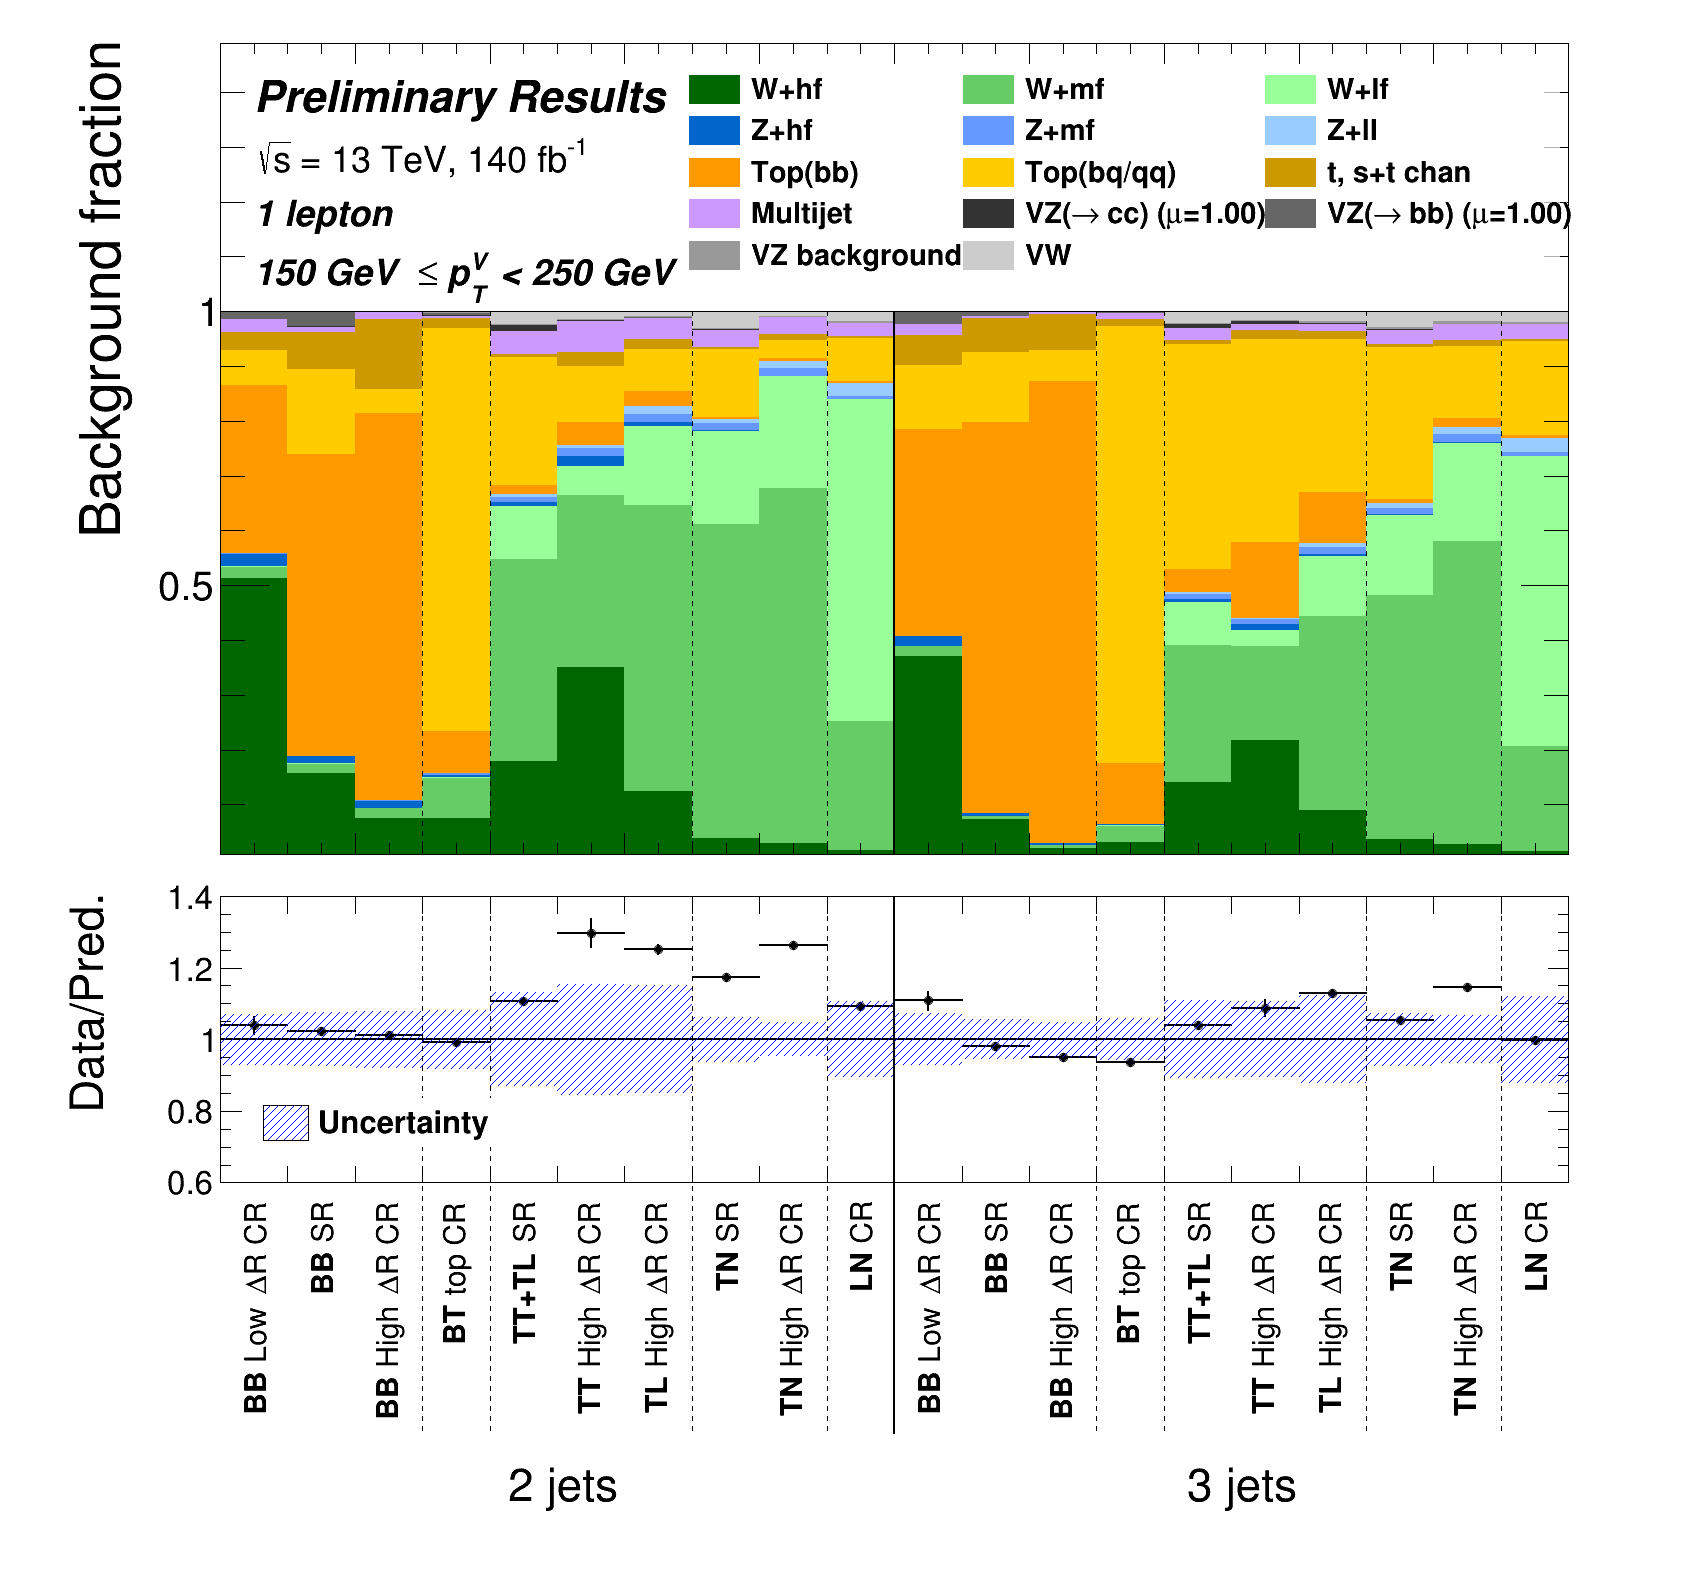
\includegraphics[width=\textwidth]{Images/VH/Own_fit/backCom_uncPrefit/GlobalFit_unconditional__Prefit/C_SRCRs_L1_BMax250_BMin150.png}
            \caption{1L, \ptv\ $\in$ [150, 250] GeV.}
            \label{fig:backCom_1L_2}
        \end{subfigure}
        \begin{subfigure}[b]{0.38\textwidth}
        \centering
        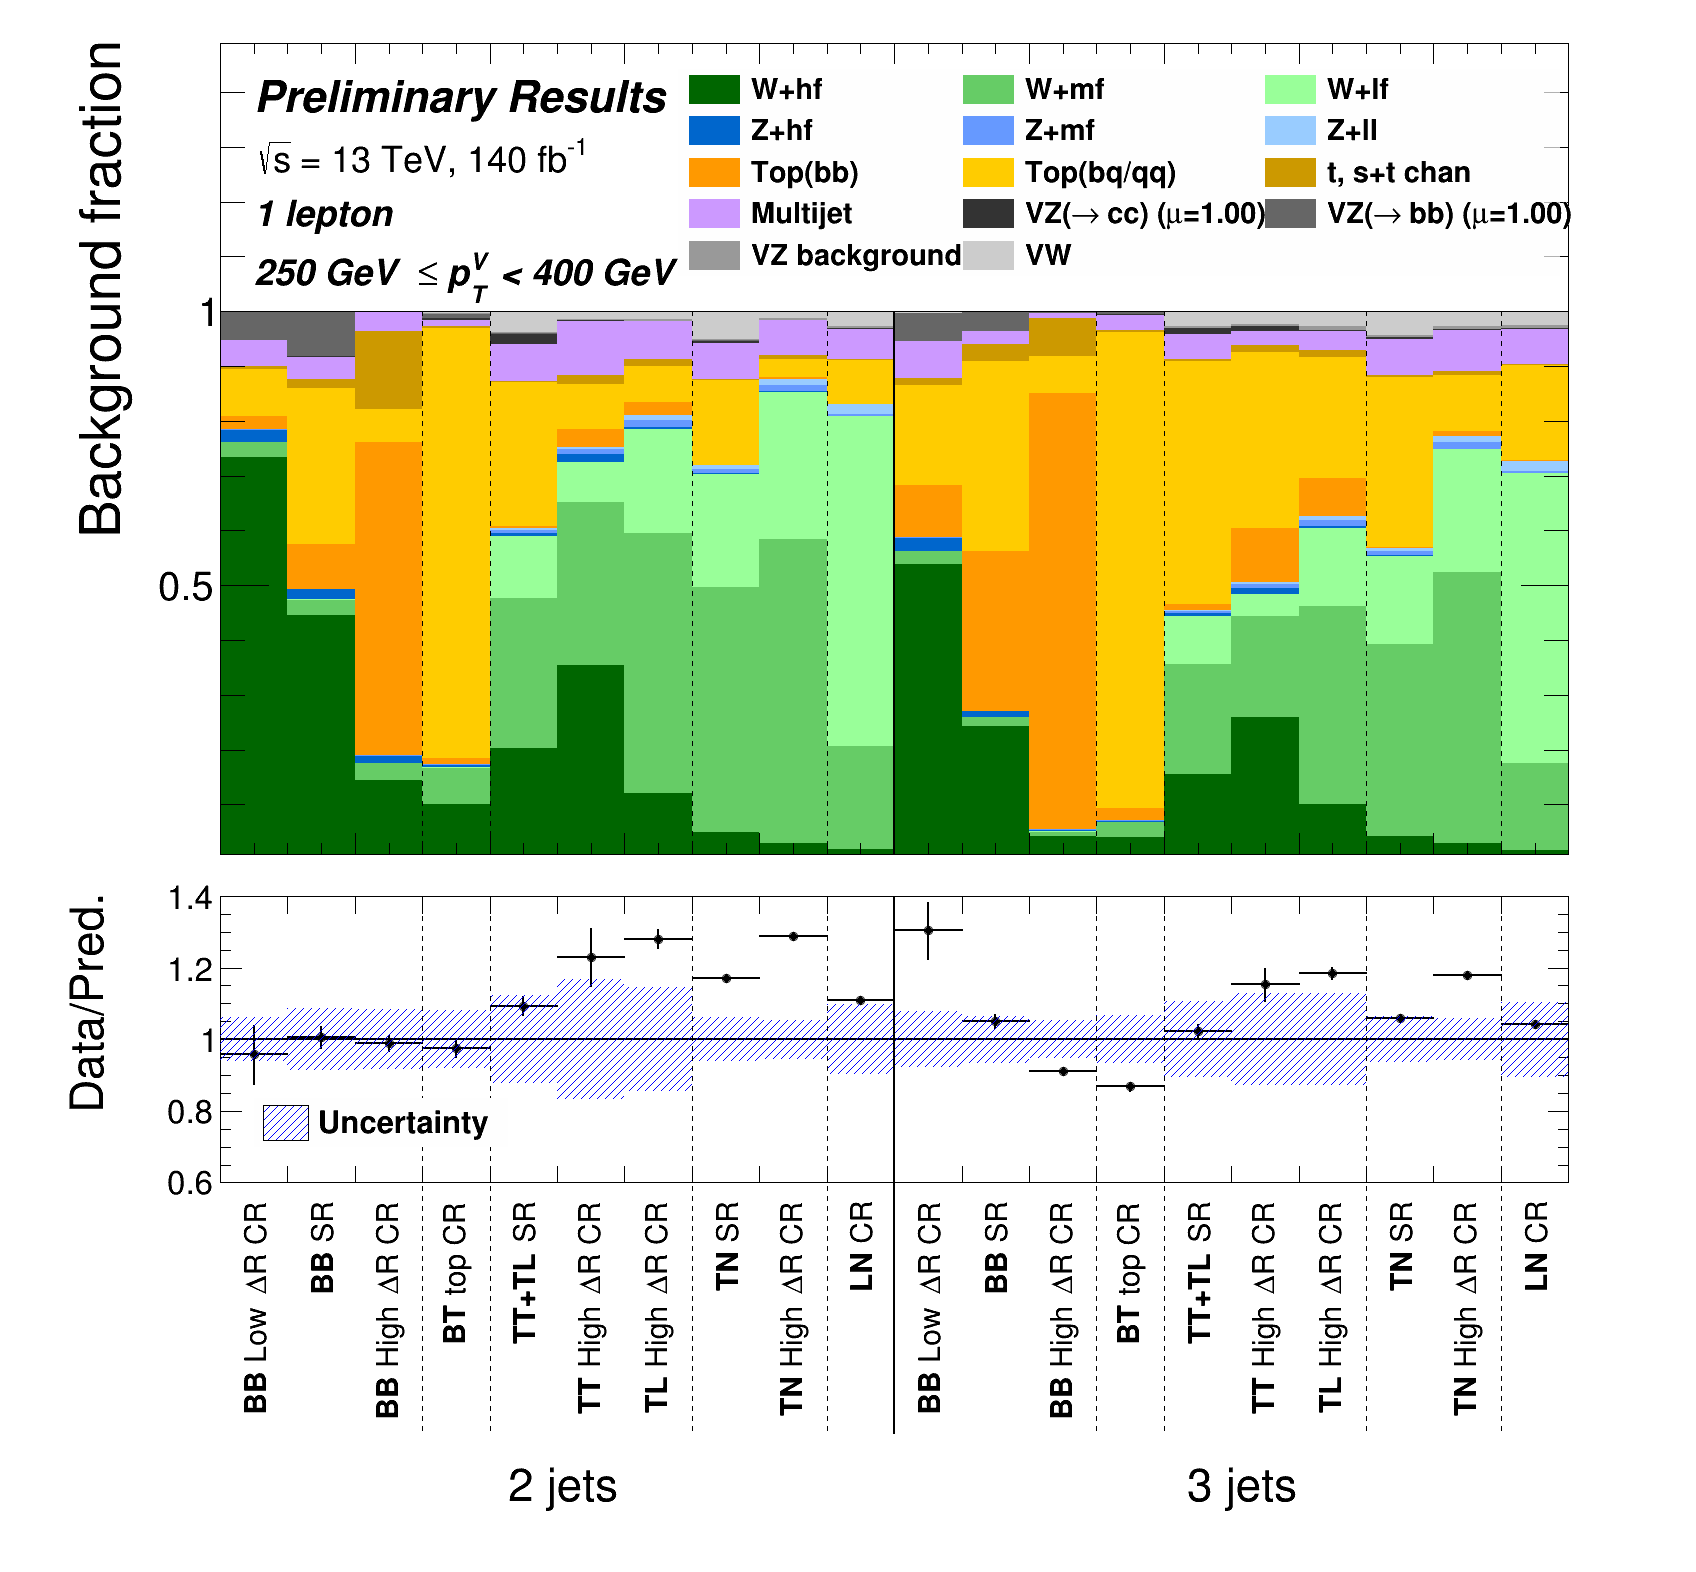
\includegraphics[width=\textwidth]{Images/VH/Own_fit/backCom_uncPrefit/GlobalFit_unconditional__Prefit/C_SRCRs_L1_BMax400_BMin250.png}
        \caption{1L, \ptv\ $\in$ [250, 400] GeV.}
        \label{fig:backCom_1L_3}
        \end{subfigure} 
    }   \\
    %\hspace{-2cm}
    \makebox[\linewidth][c]{%
        \begin{subfigure}[b]{0.38\textwidth}
            \centering
            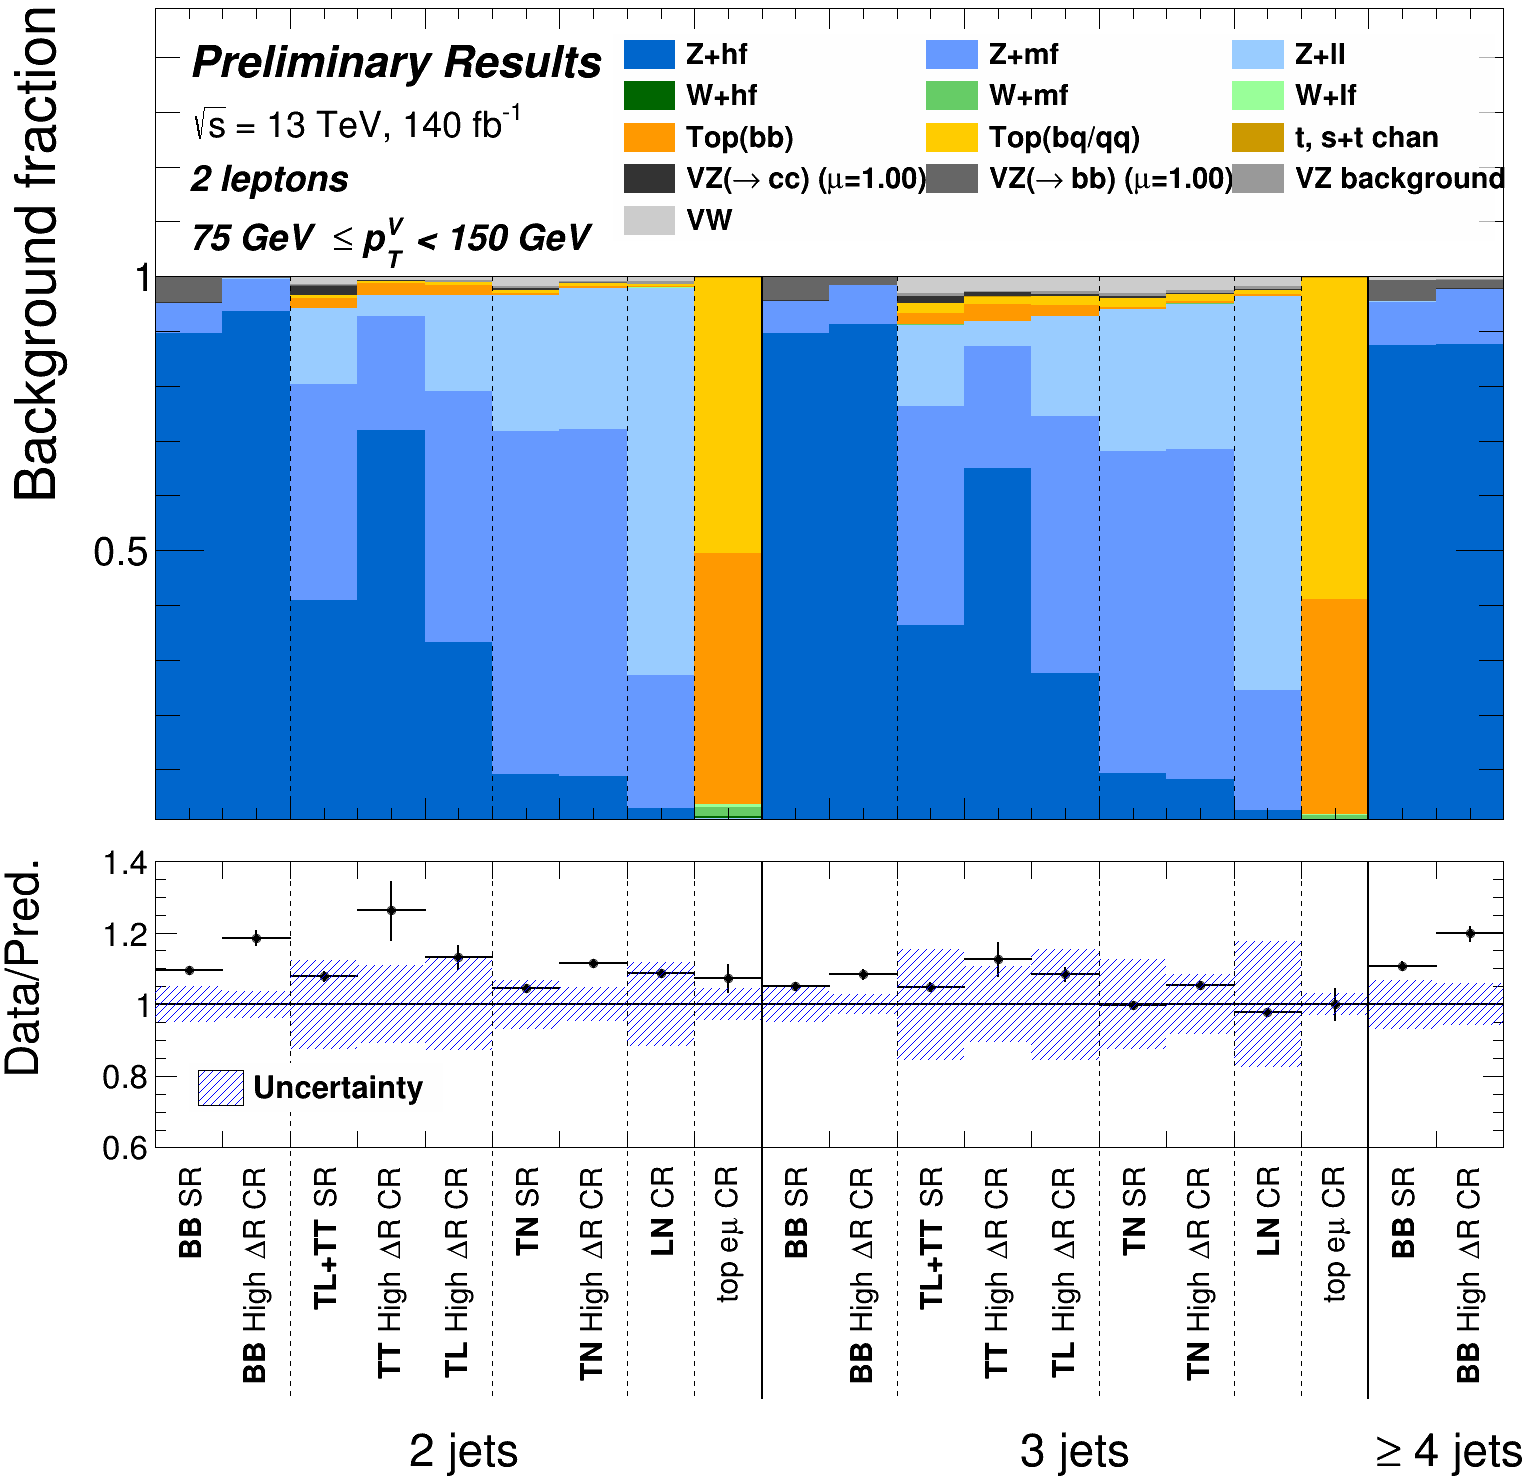
\includegraphics[width=\textwidth]{Images/VH/Own_fit/backCom_uncPrefit/GlobalFit_unconditional__Prefit/C_SRCRs_L2_BMax150_BMin75.png}
            \caption{2L, \ptv\ $\in$ [75, 150] GeV.}
            \label{fig:backCom_2L_1}
        \end{subfigure}
        \begin{subfigure}[b]{0.38\textwidth}
            \centering
            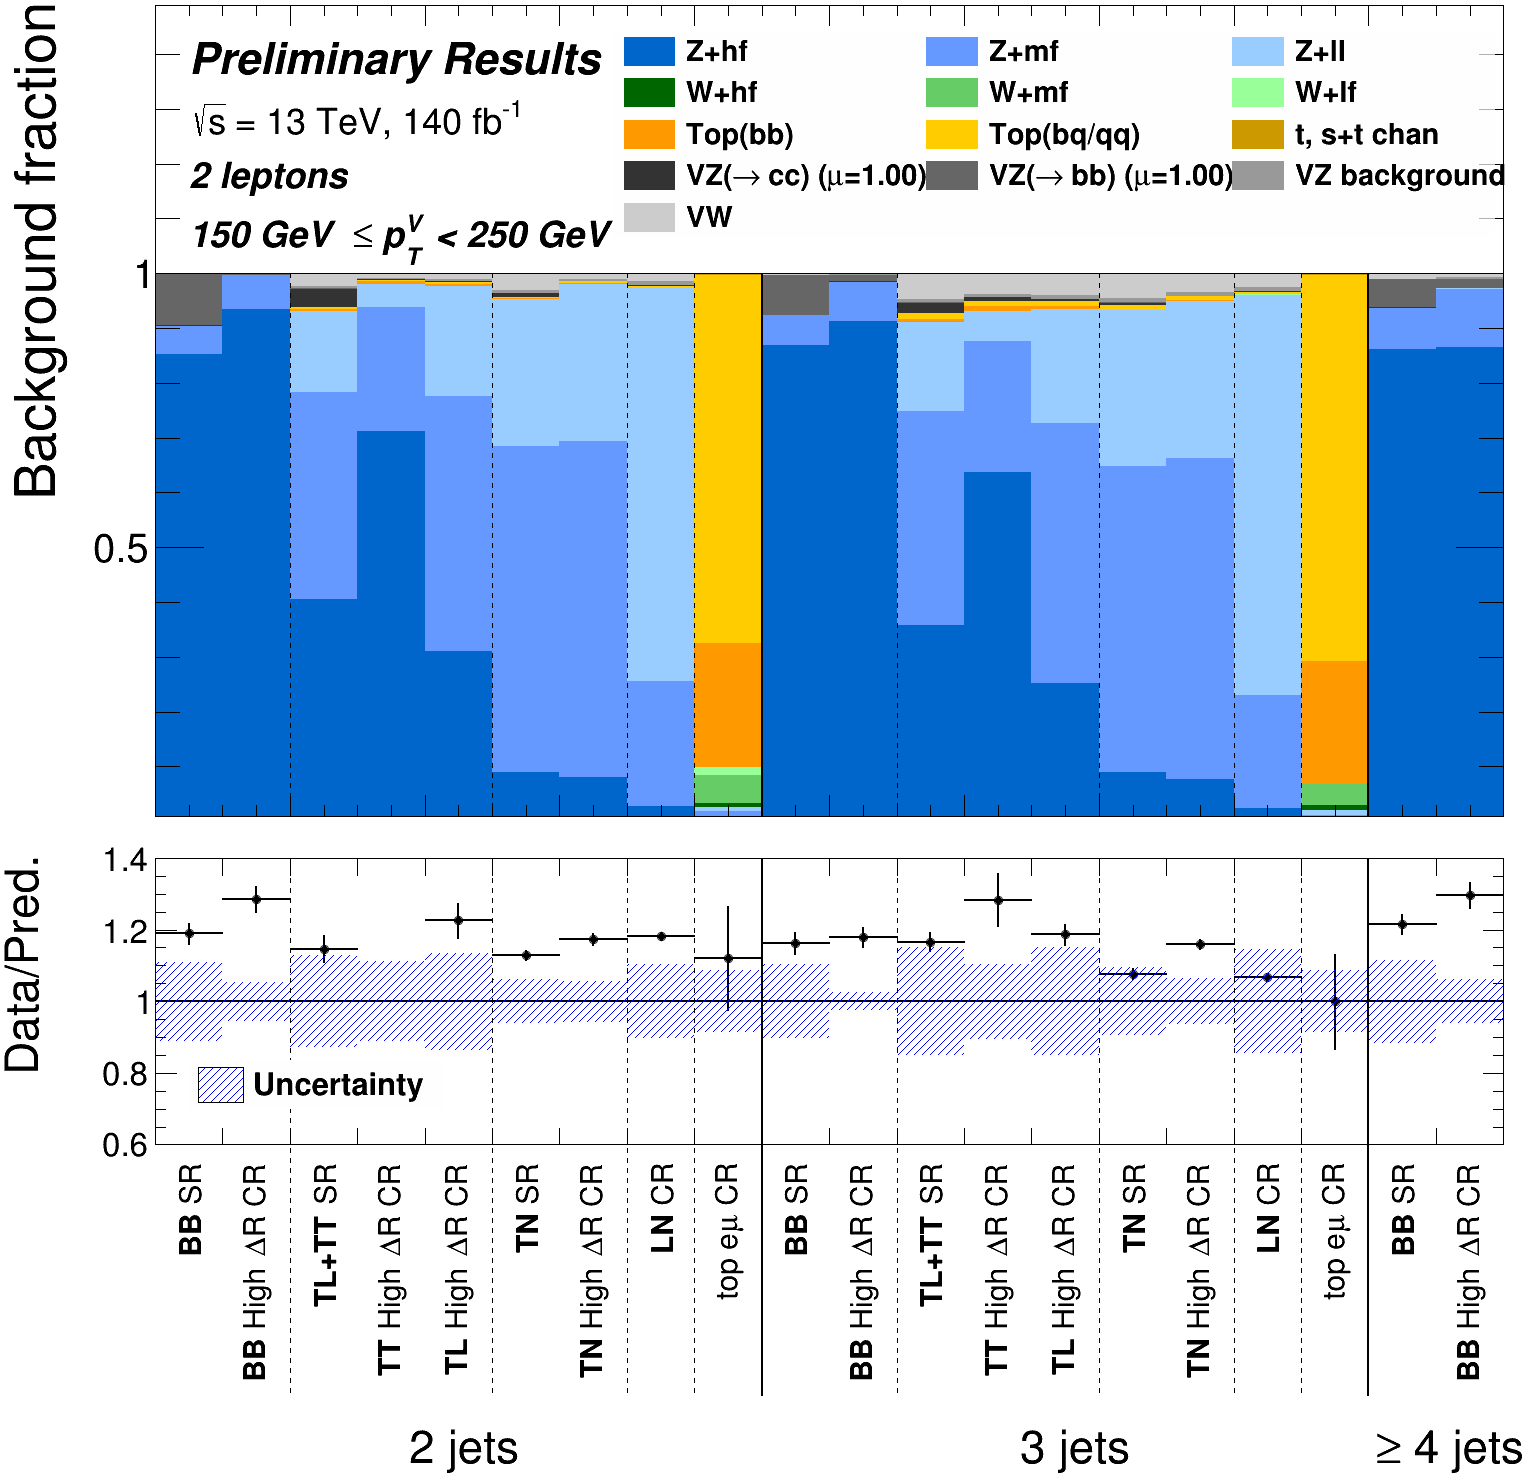
\includegraphics[width=\textwidth]{Images/VH/Own_fit/backCom_uncPrefit/GlobalFit_unconditional__Prefit/C_SRCRs_L2_BMax250_BMin150.png}
            \caption{2L, \ptv\ $\in$ [150, 250] GeV.}
            \label{fig:backCom_2L_2}
        \end{subfigure}
        \begin{subfigure}[b]{0.38\textwidth}
            \centering
            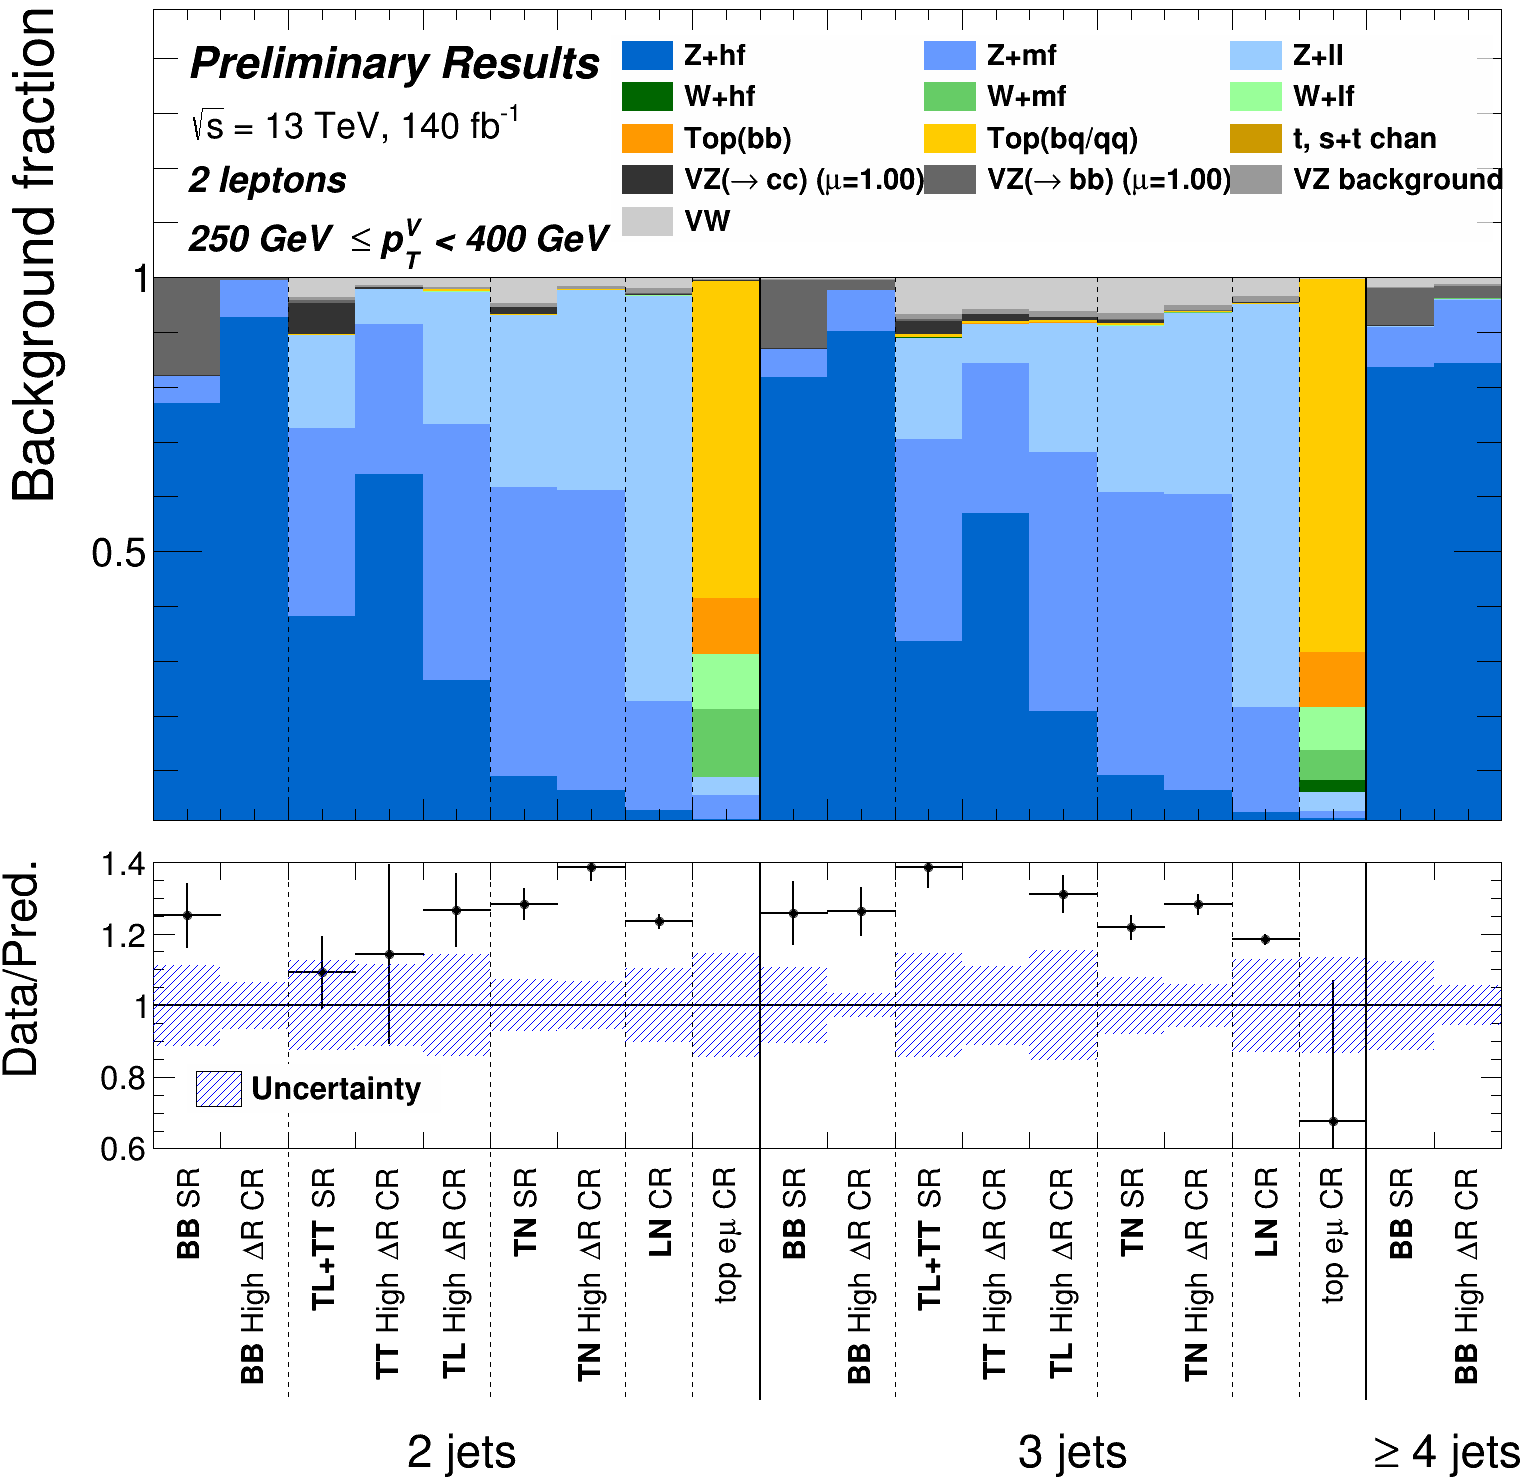
\includegraphics[width=\textwidth]{Images/VH/Own_fit/backCom_uncPrefit/GlobalFit_unconditional__Prefit/C_SRCRs_L2_BMax400_BMin250.png}
            \caption{2L, \ptv\ $\in$ [250, 400] GeV.}
            \label{fig:backCom_2L_3}
        \end{subfigure} 
    }
    \caption{The background composition of the different analysis regimes and lepton channels, with the data - Monte Carlo prefit agreement.}
    \label{fig:backCom}
\end{figure} 
  
\subsection{Modelling Strategy}\label{sec-modStrat}
The combined analysis adopts some common strategy to model the backgrounds and signal, which are described in this section before reviewing speficities adopted for each process. A guideline for the modelling is to treat backgrounds coherently across analysis regimes and correlate uncertainties between the \vhb and \vhc side when possible. The normalisations of all major backgrounds, $V+$jets and Top, are free to float in the fit, with \gls{fn} split by \ptv\ and jet multiplicity when the statitics allows. Minor backgrounds are fixed at \gls{mc} predictions with a normalisation uncertainty. To account for \gls{mc}-generator modelling uncertainty, comparisons of the nominal samples to alternative samples introduced in section \ref{sec-datasets} and summarised in Table \ref{tab:summary_altsamples} is performed. For each process, the uncertainties are split into normalisation, relative acceptance, and shapre uncertainties.  % Check top s is treated like that;

\begin{table}[!h]
    \centering
    \begin{tabular}{llll}
      \hline \hline 
      Sample & Nominal Generator & Alternative Generators & systematic effects\\
      \hline
      \vhb & \textsc{Powheg} + \textsc{Pythia 8} & \textsc{Powheg} + \textsc{Herwig 7} & $\mu_R$, $\mu_F$, \gls{isr}, \gls{fsr}, \gls{pdf}\\
      \hline
      \vhc & \textsc{Powheg} + \textsc{Pythia 8} & \textsc{Powheg} + \textsc{Herwig 7} & $\mu_R$, $\mu_F$, \gls{isr}, \gls{fsr}, \gls{pdf} \\
      \hline
      $V$+jets & \textsc{Sherpa} 2.2.11 & \textsc{MadGraph5 FxFx}, & $\mu_R$, $\mu_F$, \gls{pdf}, \\
                                            & & \textsc{Sherpa} 2.2.1 & \gls{ew} corrections \\
      \hline
      \ttb\ \& & \textsc{Powheg}+\textsc{Pythia} 8 & \textsc{Powheg}+\textsc{Herwig} 7,  & Additional \gls{isr}, \gls{fsr}, \\
      single-top &  & \textsc{MadGraph5}+\textsc{Pythia} 8  & DS/DR (single-top $Wt$) \\
      \hline
      Diboson & \textsc{Sherpa} 2.2.11  & \textsc{Powheg}+\textsc{Pythia} 8, \textsc{Sherpa} 2.2.1 & $\mu_R$, $\mu_F, \gls{pdf}$,\\
       &  & & \gls{ew} corrections\\
      \hline \hline 
    \end{tabular}
    \caption{Summary of nominal and alternative samples in the analysis. Alternative samples include different generator and systematics effects from modification to the nominal setup.}
    \label{tab:summary_altsamples}
  \end{table}
  
  
\paragraph{Normalisation uncertainties:} an overall uncertainty on the yield of a process, computed in and applied to all regions.

\paragraph{Acceptance uncertainties:} relative acceptance uncertainties cover possible change in the distributions of events across the different regions of the analysis phase space. They account for migration of events between regions and are assessed by observing the change of ratio of events between regions when switching generated samples. The prior on these uncertainties are calculated with the double ratio of Equation \ref{eq-doubleRatio}:
\begin{equation}\label{eq-doubleRatio}
    \text{Acceptance Unc}_i = \frac{\text{Acceptance}[\text{Cat.}^B (\mathrm{alternative}_i\mathrm{\,\,MC})]}{\text{Acceptance}[\text{Cat.}^A (\mathrm{alternative}_i\mathrm{\,\,MC})]} \Bigg/ \frac{\text{Acceptance}[\text{Cat.}^B (\mathrm{nominal\,\,MC})]}{\text{Acceptance}[\text{Cat.}^A (\mathrm{nominal\,\,MC})]},
\end{equation}
where category $A$ ($\text{Cat.}^A$) is the highest purity region and $B$ ($\text{Cat.}^B$) is the region studies. If several alternative generators are used ($i > 1$), the respective double-ratio are summed in quadrature: \[ \text{Total Acceptance Unc} = \sqrt{\sum_i\left(\text{Acceptance Unc}_i\right)^2}.\] If the extrapolation is across several regions $A$, $B$, $C$ of decreasing purity order, the acceptance ratio is decomposed two extrapolations: a first one from $A \rightarrow B+C$, with an additional $B \rightarrow C$ uncertainty. 

\paragraph{Shape uncertainties:} the \gls{bdt} shapes and other kinematic distributions of the processes in the different regions are given some flexibility in the fit by introducing shape uncertainties derived from a comparison of the nominal to the alternative samples. The combined analysis introduces the novel \gls{carl} technique to derive a reweighted shape uncertainty using a neural network \cite{carl}. A \gls{dnn} is trained to discriminate the nominal from an alternative, with the process repeated for each individual alternative sampels. The \gls{carl} output scores is the probability for an event to belong to the alternative sample, which can be used to reweight the nominal distribution into the alternative distribution. The advantage of this technique is the reweighted nominal distributions benefit from a much larger statistics than the alternative ones, thus smoothing out statistical fluctuations and reducing the \gls{mc} statistics uncertainties. An example of such a derived \gls{carl} shape uncertainty for the single-top $Wt$ process \textsc{MadGraph5\_aMC@NLO} in 1-lepton is presented in Figure \ref{fig:carl:resolved_closure_stopWt}. Additional shape uncertainties from \gls{ew} corrections, \gls{qcd} scales, a \ptv\ \textsc{Sherpa} 2.2.1, parton shower alternative for the signal samples, and a shape uncertainty for single-top $Wt$ DS/DR shape are directly derived.

\begin{figure}[!htbp]
    \centering
      \subfloat[SR BDT distribution.]{
        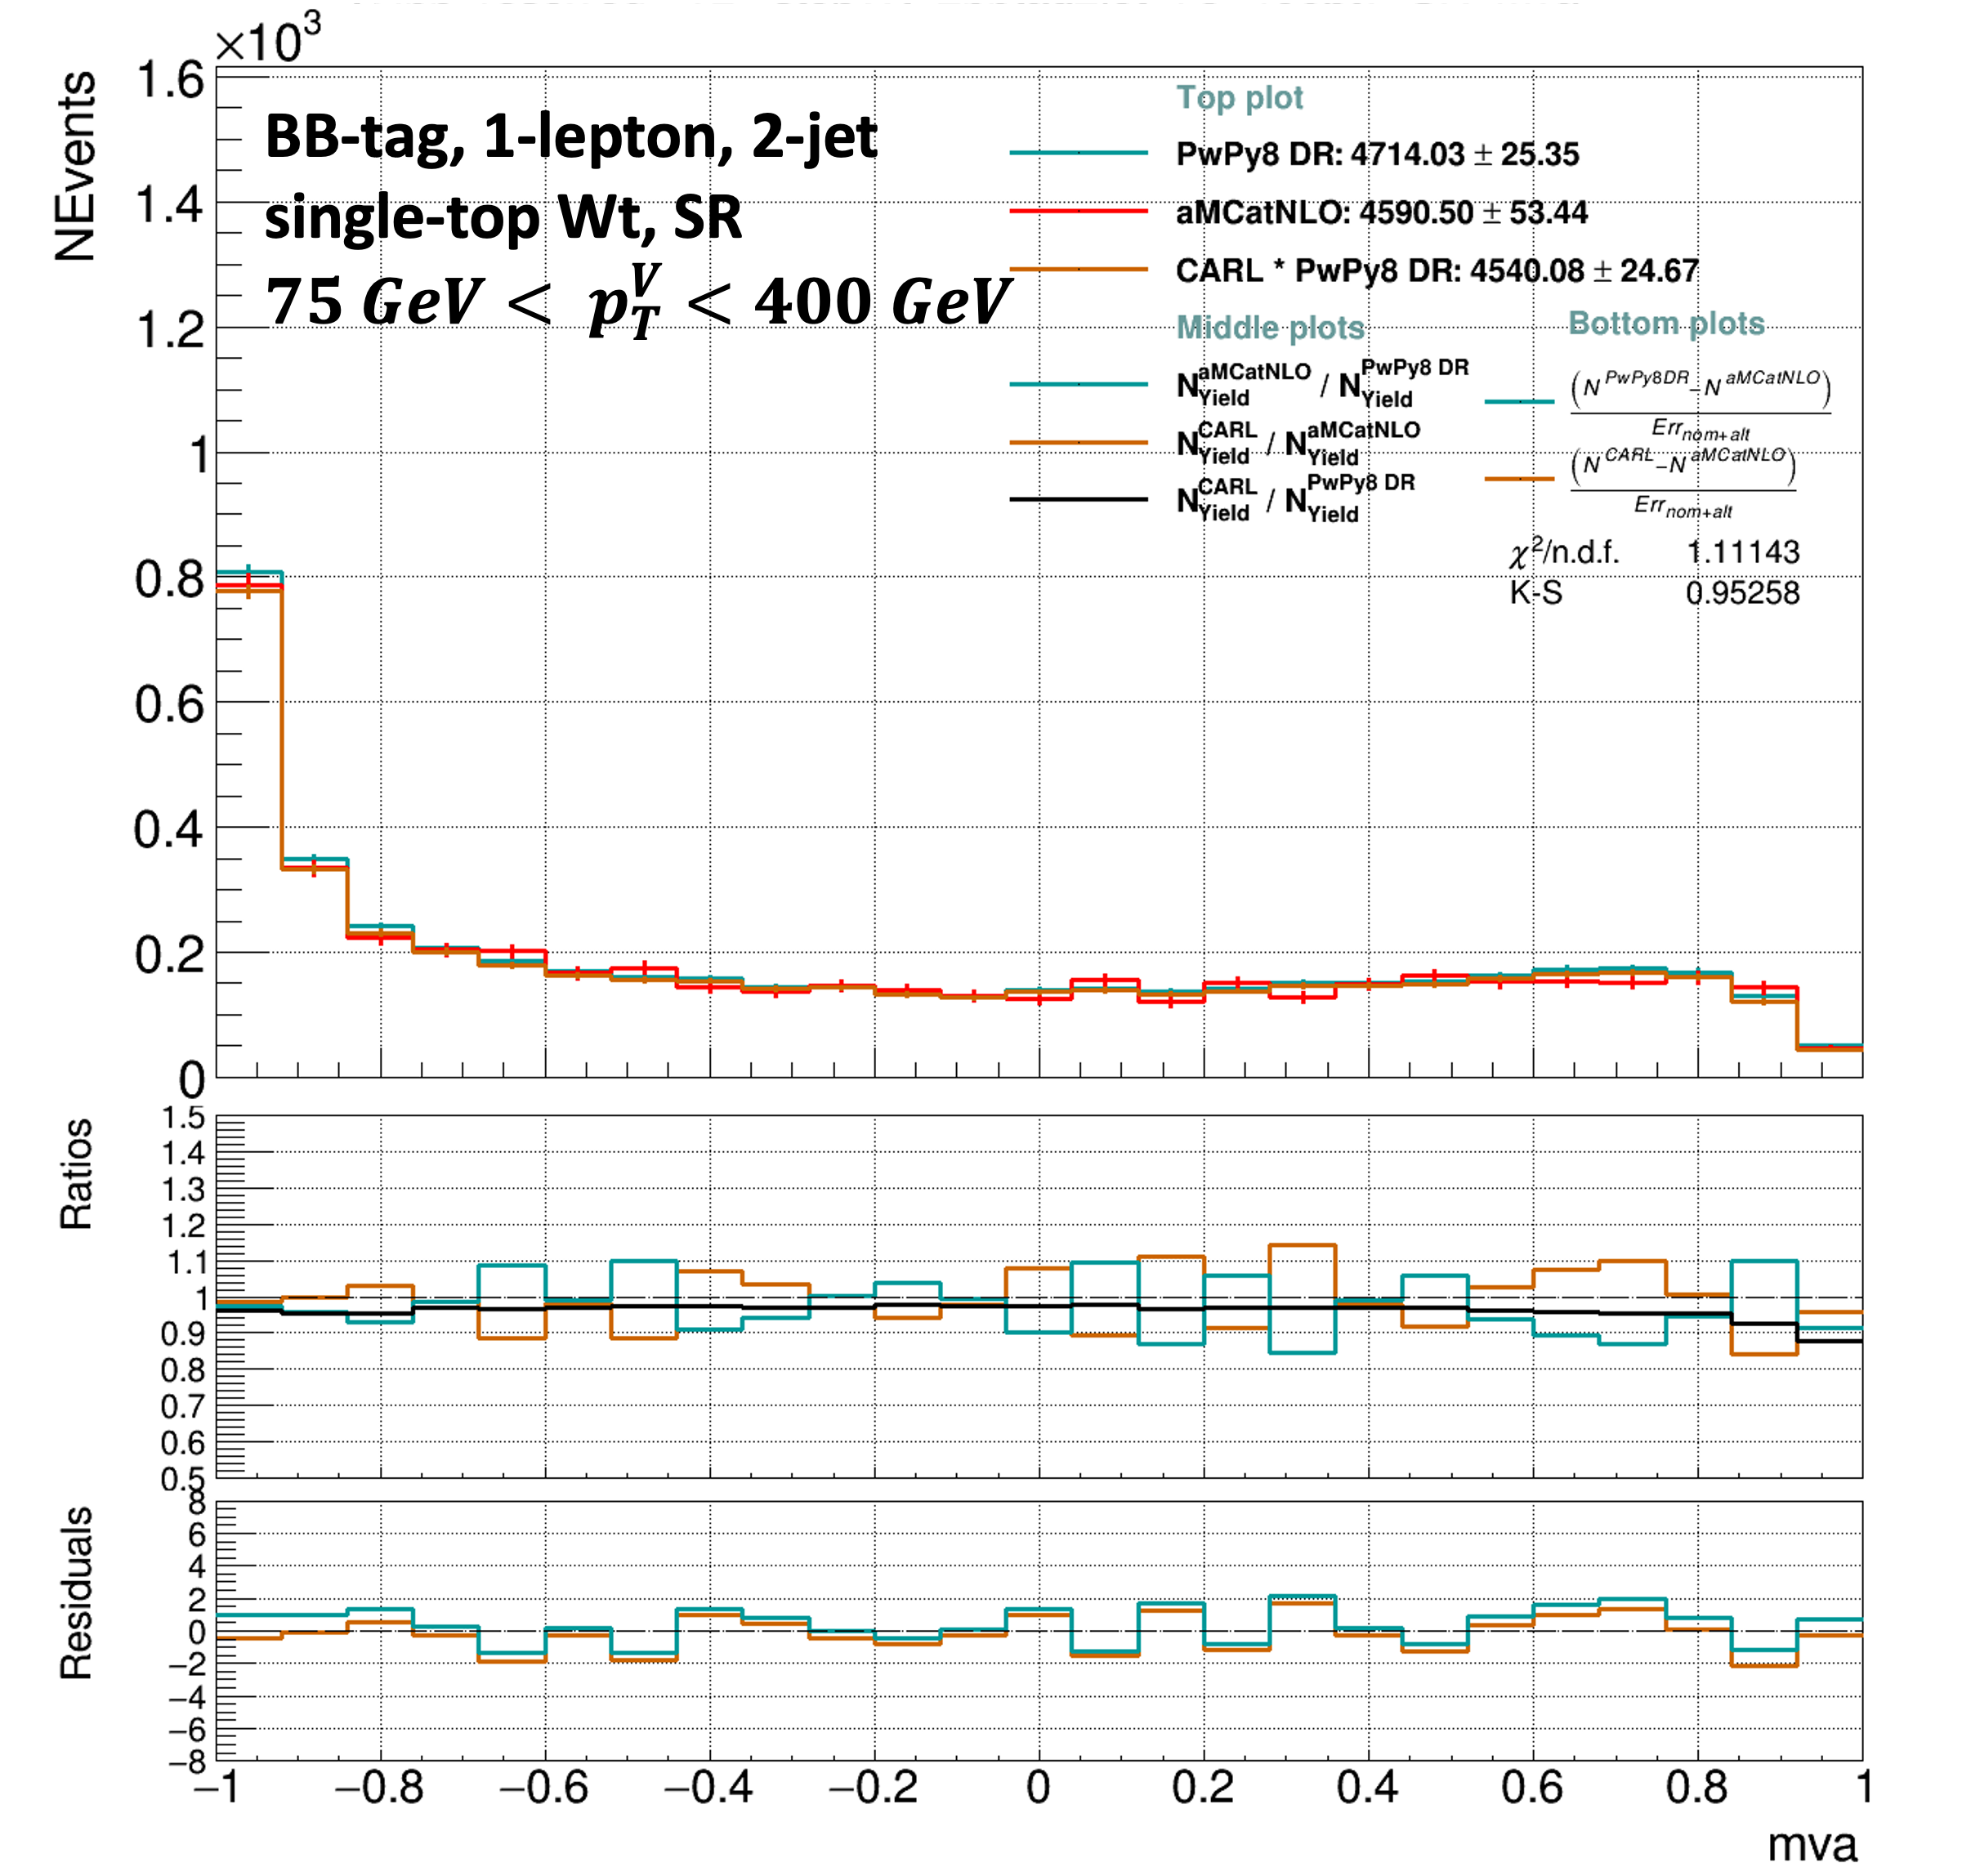
\includegraphics[width=0.48\textwidth]{Images/VH/Carl/wt/sr.png}
      }
      \subfloat[\highdr\ CR $m_{bb}$ distribution.]{
        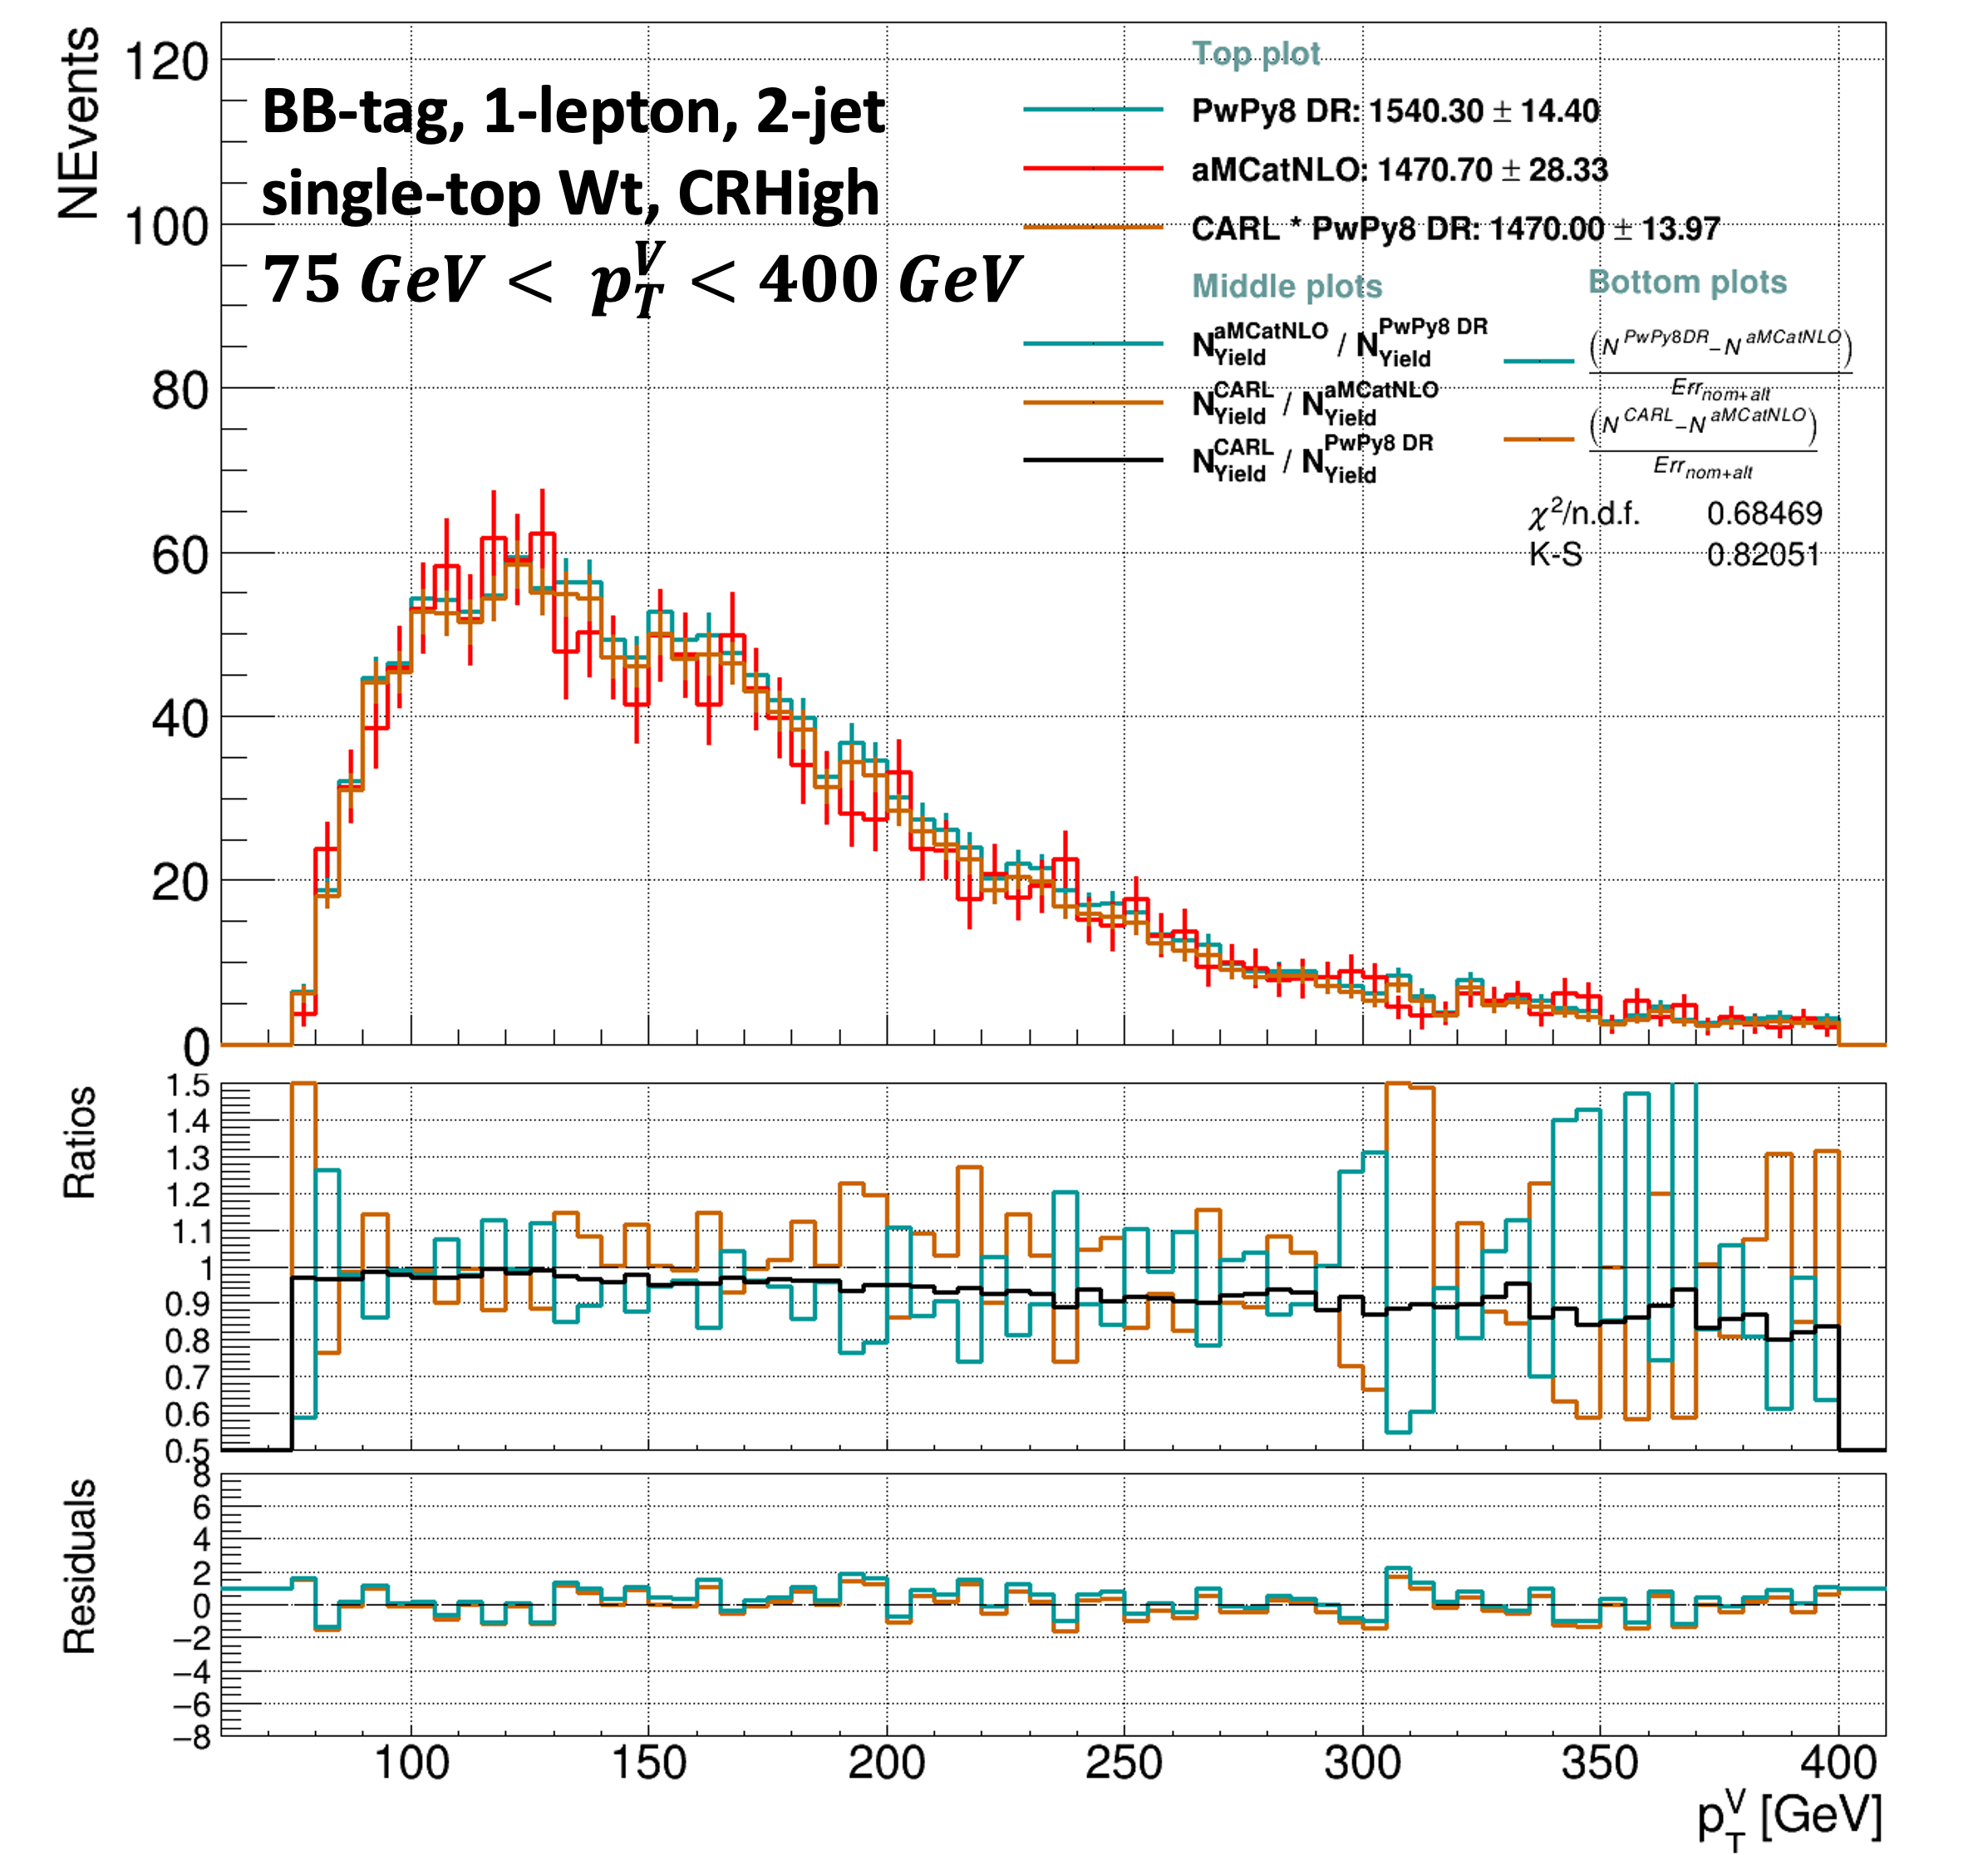
\includegraphics[width=0.48\textwidth]{Images/VH/Carl/wt/crhigh.png}
      }
      \caption{CARL closure plots, between the nominal \textsc{Powheg}\textsc{Pythia}8 (PwPy8) (with the DR scheme) and the alternative \textsc{MadGraph5\_aMC@NLO} (aMCatNLO - more details in Section \ref{subsec-vh-top-samples}), for the single-top $Wt$ production in \vhb, 1-lepton, 75 GeV < \ptv\ < 400 GeV, and 2 jets. The CARL interpolation (orange) of the nominal (blue) into the alternative (red) is smoother and with lower MC-stats. uncertainty. Top plots show the distributions, middle plots the ratios, and bottom plots the residuals.}
      \label{fig:carl:resolved_closure_stopWt}
  \end{figure}
  
  A summary of the signal and background modelling systematics considered is presented in Figure \ref{tab:syst_summary}.

  \begin{table}
    \scriptsize
    \resizebox{\textwidth}{!}{
    \begin{tabular}{l c c}
        \hline \hline
        Uncertainties & Resolved \vhbc & Boosted \vhb \\
        \hline
        \textbf{Signal} \\
        $qqWH$ / $qqZH$ / $ggZH$ normalisation/acceptance & \multicolumn{2}{c}{Values from previous analyses \cite{ATLAS:2020fcp, ATLAS:2020jwz, Collaboration:2721696}} \\
        $H\to bb$ BR & \multicolumn{2}{c}{1.61\%} \\
        $H\to cc$ BR & \multicolumn{2}{c}{From +5.53\% to -1.99\%} \\
        \hline
        \textbf{$Z$+jets} \\
        $Z+$\textit{hf} normalisation & \multicolumn{2}{c}{Floating} \\
        $Z+$\textit{mf} normalisation & Floating & 35\% \\
        $Z+$\textit{lf} normalisation & Floating & 35\% \\
        $Z+$\textit{hf} flavour composition ratio & 8\% - 12\% & 6\% - 9\% \\
        $Z+$\textit{mf} flavour composition ratios & 4\% - 10\% & 6\% - 9\% \\
        High-$\Delta R$ CR to SR & 5\% - 30\% & - \\
        topCR-SR extrapolation ratio & - & 15\% - 25\% \\
        2L to 0L acceptance ratio & 2\% - 10\% & 3\%\\
        \ptv\ extrapolation & - & 15\% \\
        \hline
        \textbf{$W$+jets} \\
        $W+$\textit{hf} normalisation & \multicolumn{2}{c}{Floating} \\
        $W+$\textit{mf} normalisation & Floating & 36\% \\
        $W+$\textit{lf} normalisation & Floating & 38\% \\ % TODO in 1L < 150 GeV it's fixed at 25\% norm unc.
        $W+$\textit{hf} flavour composition ratios & 4\% - 25\% & 11\% \\
        $W+$\textit{mf} flavour composition ratios & 14\% - 29\% & 9\% - 15\% \\
        $W+$\textit{lf} flavour composition ratios & 9\% & - \\
        High / Low-$\Delta R$ CR-SR extrapolation ratios & 2\% - 63\% & - \\
        topCR-SR extrapolation ratio & - & 16\% - 27\% \\
        1L to 0L acceptance ratio & 3\% - 30\% & 20\% \\
        \ptv\ extrapolation & - & 3\% \\
        $N_{\mathrm{jet}}$ extrapolation & 12\% - 20\% & - \\
        \hline
        \textbf{Top (\ttb\ + single-top $W$t) 0L \& 1L resolved} \\
        Top$(bb)$ normalisation & Floating &  - \\
        Top$(bq/qq)$ normalisation & Floating & - \\
        Flavour acceptance ratios & 5\% - 10\% & - \\
        1L to 0L acceptance ratios & 2\% - 8\% & - \\
        High / Low-$\Delta R$ CR-SR extrapolation ratios & 2\% - 10\% & - \\
        $Wt$ / \ttb\ ratios & 12\% - 48\% & - \\
        \hline
        \textbf{Top (\ttb\ + single-top $W$t) 2L resolved} \\
        Normalisation in \vhc & Floating & - \\
        Normalisation in \vhb^* & 0.08\%   & - \\
        \hline
        \textbf{Single-top ($t$-channel) 0L \& 1L resolved} \\
        Normalisation $s$ - $t$ & 4.6\% - 17\% & - \\
        High / Low-$\Delta R$ CR-SR extrapolation ratios & 3\% - 17\% & - \\
        \ptv\ extrapolation ratios & 7\% - 15\%  & - \\
        \nj\ acceptance ratios & 15\% & - \\
        1L to 0L acceptance ratio & 6\% & - \\
        \hline
        \textbf{\ttb\ and single-top boosted} \\
        top (\ttb\ + $Wt$) normalisation & - & Floating \\
        single-top $s$ and $t$ normalisations & - & 4.6\% - 10\%\\
        1L to 0L acceptance ratio top & - & 6\% - 20\% \\
        topCR-SR acceptance ratio top & - & 10\%\\
        $Wt$ / \ttbar ratio & - & 22\% - 36\%
        \hline
        \textbf{Diboson} \\
        $WW$ / $ZZ$ / $WZ$ normalisation & 16\% / 17\% / 19\% &  16\% / 17\% / 27\%\\
        $ggVV$ normalisation & \multicolumn{2}{c}{30\%} \\
        Lepton channel acceptance & 2\% - 23\% & 7\% \\
        $N_{\mathrm{jet}}$ acceptance & 10\% - 30\% & - \\
        % VZ HP-LP acceptance & - & 10-15\% \\
        \ptv\ acceptance & 3\% - 16\% & 8\% - 40\% \\
        SR / CR acceptance & 6\% - 16\% & - \\
        STXS like binning acceptance & - & 1.2\% - 42.2\% \\ % TODO Need to find this for resolved
        \hline
        \textbf{Multi-jet (1L)$^*$} \\
        Normalisation & 20\% - 100\% & - \\
        \hline \hline
    \end{tabular}
    }
    \caption{Summary of the modelling systematic uncertainties considered. The values given refer to the size of the uncertainty affecting the yield of each background. Uncertainties in the shapes of the distributions are not
    shown but taken into account for all backgrounds. $^*$The multijet background in the 1L channel and the top background in the 2L $BB$-tagged resolved are data driven.}
    \label{tab:syst_summary}

\end{table}
 % TODO, need to check the signal uncerrtainties

  \subsection{Signal Modelling}\label{sec-modSignal}
  The signal is coherently modelled across regimes and targeted final state. The three main signal productions $qq \rightarrow WH$, $q\bar{q} \rightarrow ZH$, and $gg \rightarrow ZH$ are modelled seperately, with uncertaintyies modelling the production and the decay mode of the Higgs into $b\bar{b}$ or $c\bar{c}$. These uncertainties cover:
  \begin{itemize}
    \item \textit{\gls{qcd} scale uncertainties:} the most important in the theoretical prediction of the $VH$ production cross-section, obtained by varying the renormalisation and factorisation scales $\mu_R$ and $\mu_F$. They are considered as shape uncertainties and uncertainties covering the inclusive cross-section and parametising migration across \ptv\ and jet multiplicity bins, following Ref \cite{ATL-PHYS-PUB-2018-035}.
    \item \textit{\gls{pdf} + $\alpha_s$ uncertainties}: alternative parton distributions from the \textsc{PDF4LHC15\_30} modifying the $VH$ cross-sections in \gls{stxs} bins are considered, with $\alpha_s$ at the $Z$-mass varied within uncertainties \cite{Butterworth:2015oua}.
    \item \textit{\gls{ew} corrections}: \ptv\ distribution uncertainties on the NLO electroweak corrections due to NNLO effects. 
    \item \textit{Branching ratio}: a theoretical uncertainty of 1.61\% on the $H \rightarrow{b\bar{b}}$ branching ratio and an uncertainty of -1.99\% to +5.53\% for the $H \rightarrow{c\bar{c}}$ branching ratio are used \cite{LHCHiggsCrossSectionWorkingGroup:2016ypw}. The $ZH$ ($WH$) cross-sections cover 96.52\% to 104.11\% (97.95\% to 101.98\%) of their values with introduced uncertainties.
    \item \textit{\gls{ps} and \gls{ue}}: parton shower and underlying event can affect the proprties of the $H \rightarrow b\bar{b} / c\bar{c}$ decay. Uncertainties are introduced to model these effects on the signal acceptance.
\end{itemize}

\subsection{$V+$jets Modelling}\label{sec-modVjet} % TODO boosted
The $V+$jets process is modelled seperately depending on the flavour of the reconstructed vector boson. 

\subsubsection{$Z+$jets}
This background is dominant in the 0L and 2L channels, but negligible in 1L. The background is split into different components of the flavour compositions of jets selected to form the Higgs candidate, grouping compositions with similar kinematic performance as:   
\begin{itemize}
    \item \textit{$Z+$ heavy flavours (\zhf)}: $Z+bb$ and $Z+cc$
    \item \textit{$Z+$ mixed flavours (\zmf)}: $Z+bc$, $Z+bl$, and $Z+cl$ (at least a $b$ or a $c$).
    \item \textit{$Z+$ light flavours (\zlf)}: $Z+l$.
\end{itemize}
Each grouping has itws own free floating normalisations, with \zhf\ dominant in \vhb\ and the other two components significant in \vhc. These \gls{fn}s are decorrelated in \ptv\ and jet multiplicities \nj\footnote{Except for the 2L with 75 GeV < \ptv\ < 150, where the \Vhb\ 4-jet is merged with 3-jet: to solve this, \vhb\ has an extra \vhf\ \gls{fn} for 3p-jet.}. The modelling of $Z+$jets includes several types of acceptance uncertainties that are applied in 0L and 2L:
\begin{itemize}[leftmargin=*]
    \item Channel extrapolation 2L $\rightarrow$ 0L uncertainties: for the \zhf, \zmf, and \zlf respectively. 
    \item Flavour composition uncertainties: accounting for the variation on the yields of different flavour in the combinations using the double ratio of Equation \ref{eq-doubleRatio}. These include a comparison of $cc$ to $bb$ for \zhf and of [$bc$, $bl$] to $cl$ for \zmf. They take into account \ptv\ and jet multiplicity \nj\ trends and cover the \vhb\ and \vhc\ sides of the resolved regime. 
    \item Region extrapolation uncertainties: are included to model the acceptance of different region (\gls{sr} and \gls{cr}). They are derived with the double ratio Equation \ref{eq-doubleRatio} from a high purity region to a low purity one depending on the combination:
    \begin{itemize}
        \item \zhf\ and \zmf: constrained mostly in the CRHigh and applied to the \gls{sr}. 
        \item \zlf: constrained mostly in 1 $LN$-tagged $V+l$ CR and the \gls{sr}. Applied in CRHigh. % TODO, in the text, it says that it's SR - CRHigh, but it's constrained in LN??
    \end{itemize}
\end{itemize}
The values of the acceptance uncertainties are presented in Table \ref{tbl:zjets_acc_full} of Appendix \ref{appsec-vh-backsigmod}, with a summary mentioned in Table \ref{tab:summary_altsamples}.

In addition, 4 different shape uncertainties are considered:
\begin{itemize}
    \item \gls{carl} shape: modelling the difference between \textsc{Sherpa} 2.2.11 and \textsc{MadGraph FxFx}, derived for all components and applied in all analysis regions.
    \item \textsc{Sherpa} 2.2.1 \ptv\ shape uncertainties to model the data-\gls{mc} mis-modelling of  \ptv\ in \textsc{Sherpa} 2.2.11.
    \item \gls{qcd} scale shape uncertainties by varying $\mu_R$ and $\mu_F$.
    \item \gls{ew} shape variations that are typically quite small.
\end{itemize} 

\paragraph{Boosted regime:} roughly the same modelling strategy to the resolved regime is applied, with the uncertainties fully detailed in the Appendix Table \ref{tbl:zjets_acc_fullBoos}. The \zhf\ component is left free-floating while the \zmf\ and \zlf\ components have an overall acceptance uncertainty of 35\%. The \zlf\ has no other acceptance uncertainty as it is negligible in the boosted regime. Flavour acceptance uncertainties for \zhf\ and \zmf\ are applied in 0L and 2L. The \zhf\ and \zmf\ also have channel acceptance uncertainties and \gls{sr} $\rightarrow$ topCR acceptance ratios applied in the 0L. Additional \ptv\ extrapolation uncertainties from [400, 600] GeV to $> 600$ GeV is considered in 0L and 2L. Shape uncertainties are derived similarly to the resolved regime. 

\subsubsection{$W+$jets}
The background is dominant in the 1-lepton channel with a residual contribution in 0-lepton mostly due to hadronically decaying $\tau$-lepton. It is split equivalenty to the $Z+$jets background as:   
\begin{itemize}
    \item \textit{$W+$ heavy flavours (\whf)}: $W+bb$ and $W+cc$
    \item \textit{$W+$ mixed flavours (\wmf)}: $W+bc$, $W+bl$, $W+b\tau$, $W+cl$, and $W+c\tau$ (at least a $b$ or a $c$).
    \item \textit{$W+$ light flavours (\wlf)}: $W+l$, $W+l\tau$, $W+\tau\tau$.
\end{itemize}
Each grouping has its own floating normalisation, with \whf signficant in \vhb, while \wmf and \wlf are more important in \vhc. These \gls{fn}s are decorrelated in \ptv\ and jet multiplicities \nj\footnote{The only exception is the 1L \wlf in 75 GeV < \ptv < 150 GeV, where a normalisation uncertainty of 25\% is considered.}. Acceptance uncertainties, summarised in Table \ref{tab:summary_altsamples} and listed in the Appendix Table \ref{tbl:wjets_acc_full}, are applied in 0L and 1L and include:
\begin{itemize}[leftmargin=*]
    \item Channel extrapolation 1L $\rightarrow$ 0L uncertainties: applied in 0L for the \whf, \wmf, and \wlf respectively. 
    \item Flavour composition uncertainties: include a comparison of $cc$ to $bb$ for \whf, of [$bc$, $bl$, $c\tau$, $b\tau$] to $cl$ for \wmf, and of [$l\tau$, $\tau\tau$] to $Wl$ for \wlf. They take into account \ptv\ and jet multiplicity \nj\ trends and cover the \vhb\ and \vhc\ sides of the resolved regime. 
    \item Region extrapolation uncertainties: for the different combinations:
    \begin{itemize}
        \item \whf: constrained mostly in the \gls{sr} + TopCR and the $BB$-tagged CRLow, applied to CRHigh in different \ptv\ regions. For \vhb, an extra CRLow $\rightarrow$ SR+TopCR is applied. 
        \item \wmf: constrained mostly in 2 $c$-tagged CRHigh and applied to SR+TopCR and CRLow.
        \item \wlf: constrained mostly in 1 $LN$-tagged $V+l$ CR and the SR. Applied in CRHigh. % TODO, in the text, it says that it's SR - CRHigh, but it's constrained in LN??
    \end{itemize}
    \item Jet multiplicity \nj acceptance: \gls{fn}s are left free floating in \nj (2-jet and 3-jet). For \vhb, the 4-jet category has no dedicated \gls{cr} and a 3-jet $\rightarrow$ 4-jet acceptance is applied to \whf (other components are negligible).
\end{itemize}

In addition, 4 different types of shape uncertainties are considered similarly to the $Z+$jets.

\paragraph{Boosted regime:} roughly the same modelling strategy is applied, with the uncertainties fully detailed in the Appendix Table \ref{tab:wjets_acc_fullBoos}. The \whf\ component is left free-floating while the \wmf\ and \wlf\ components have an overall acceptance uncertainty of 36\% and 38\% respectively. Flavour acceptance uncertainties are considered for \whf\ and \wmf\ from $Wbc$ (the components with $\tau$ are negligible). The different components also have channel acceptance uncertainties applied in 0L-channel and \gls{sr} $\rightarrow$ topCR acceptance ratios applied in the 0L- and 1L-channels. Additional \ptv\ extrapolation uncertainties from [400, 600] GeV to $> 600$ GeV is considered in 0L and 1L. Shape uncertainties are derived similarly to the resolved regime. 

\subsection{Top Modelling}\label{sec-modTop} 
These backgrounds adress the decay of a top-quark $t$, including the \ttb\ pair-production and the single-top $Wt$ production as well as the single-top $t$- and $s$-channels, in order of relative importance. The \ttb\ and single-top $Wt$ are combind into a \textit{Top} component in the resolved regime, while the single-top $t$- and $s$-channels are combined into an other single-top component. The Top background (throughout this chapter, Top will refer to the combination of the \ttb\ \& $Wt$ processes) in 0L and 1L are estimated from \gls{mc} and dedicated Top $BT$ control region. In the resolved regime, the Top is grouped into different components based on three flavour categories:
\begin{itemize}
    \item Top$(bb)$: mostly in the \vhb\ phase space of the signal regions and the \highdr\ \gls{cr}s thanks to the large initial angle between the emitted top-quark, passed over to the two $b$-quarks.
    \item Top$(bq)$: combinies top$(bc)$ and top$(bl)$. It is mostly in the \vhc\ phase space and is well-selected by the $BT$-tagged Top \gls{cr}.
    \item Top$(qq)$: combines top$(cc)$, top$(cl)$ and top$(ll)$. Mostly in the $TN$ and $TL$ regions of the \vhc.
\end{itemize}

\begin{figure}[!htbp]
    \centering
      \subfloat[]{
        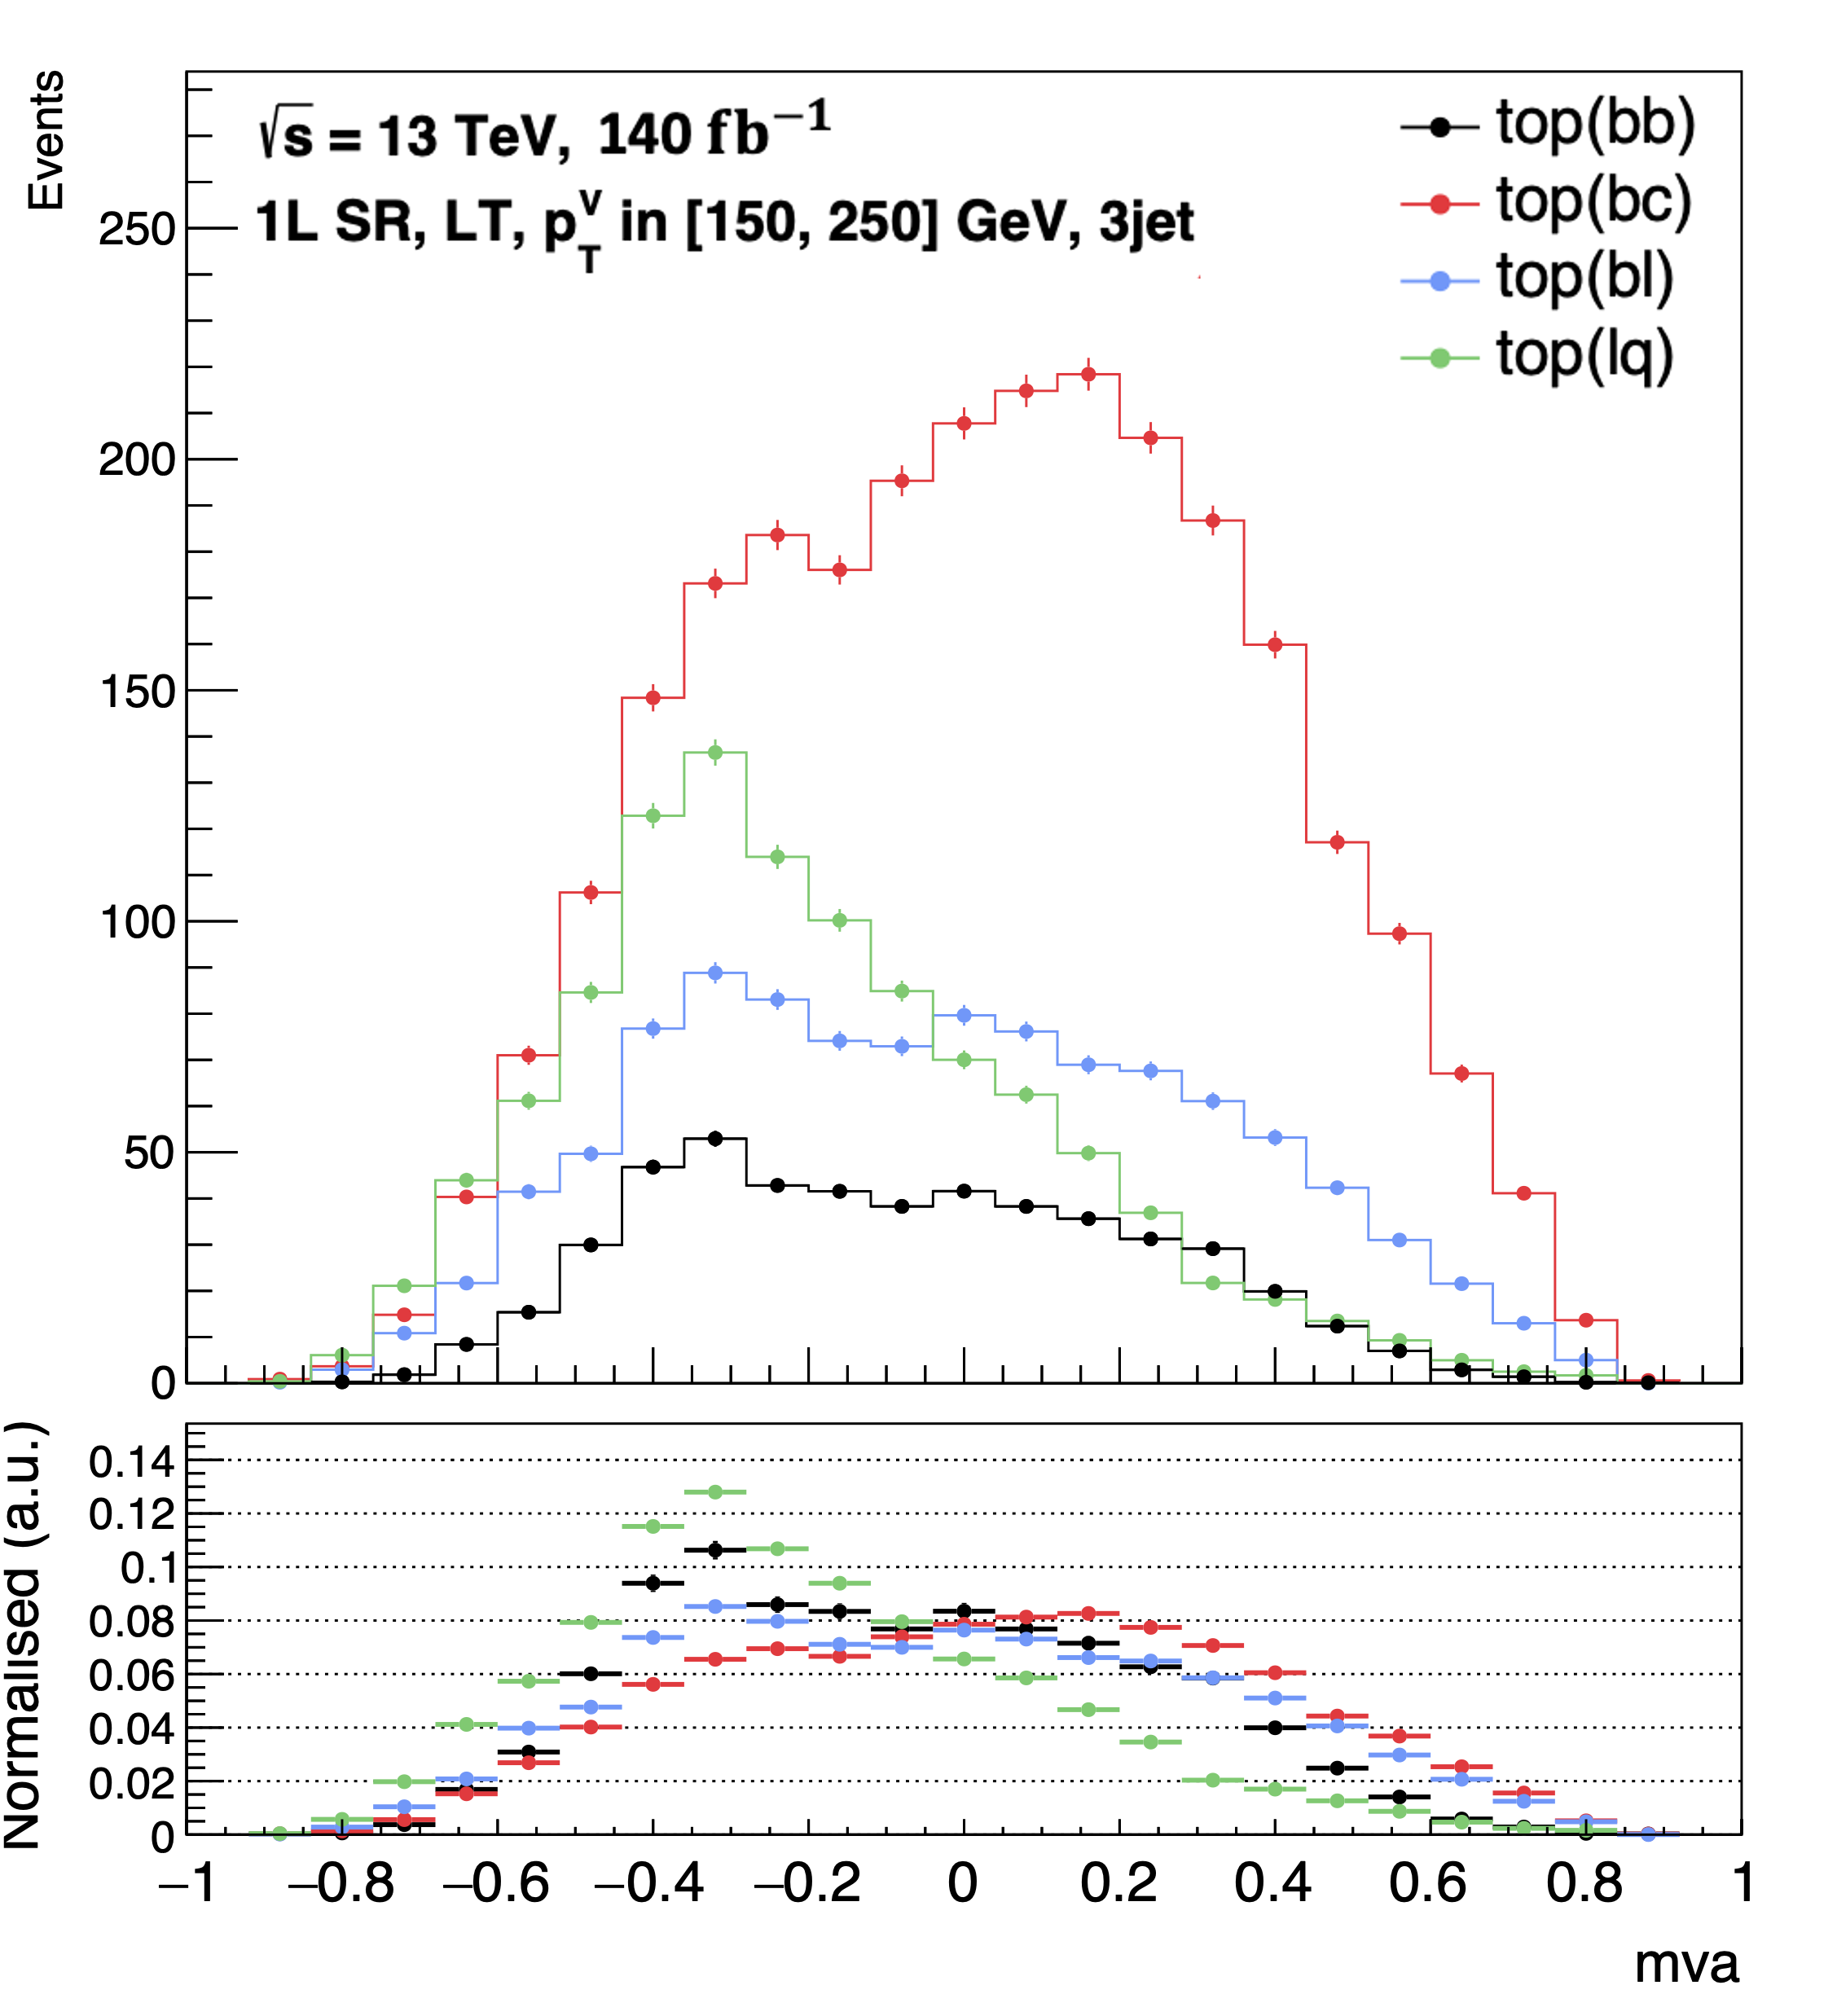
\includegraphics[width=0.45\textwidth]{Images/VH/Model/Top/TopcompoSRLT.png}
      }
      \subfloat[]{
        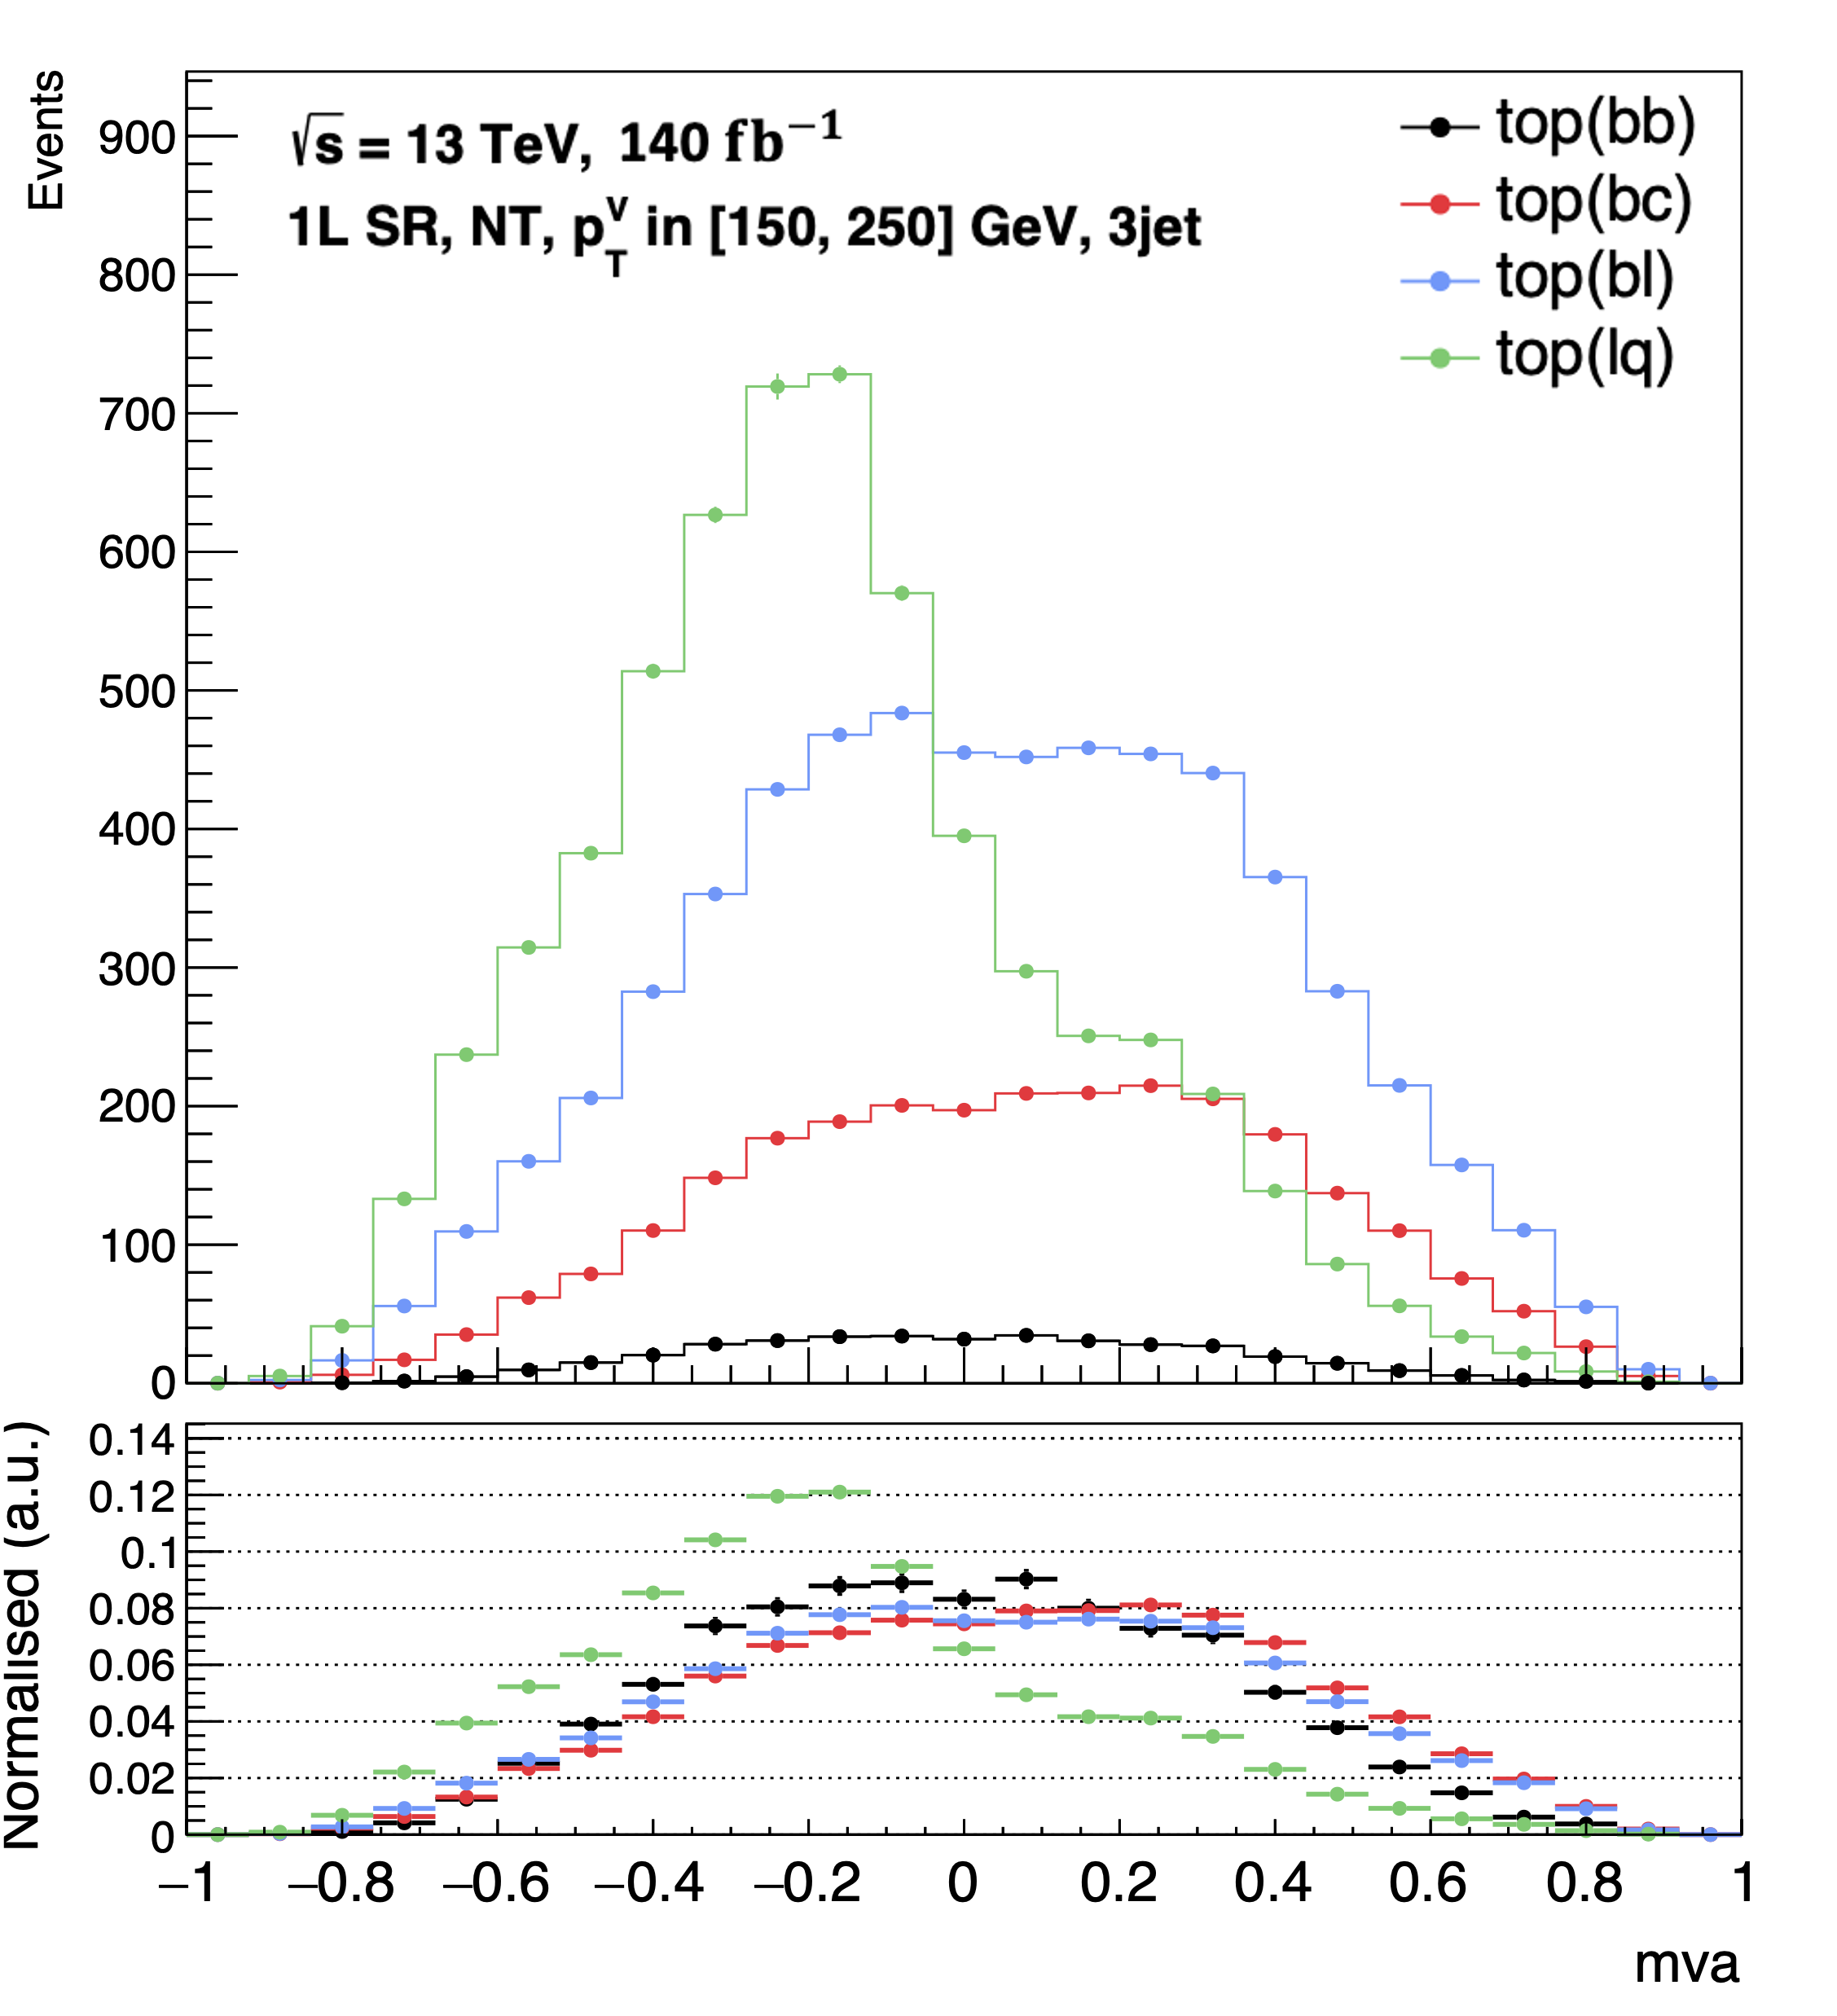
\includegraphics[width=0.45\textwidth]{Images/VH/Model/Top/TopcompoSRNT.png}
        }
      \caption{The non-rebinned MVA distribution of the top background (direct tagged) in the \vhc\ signal regions ($TN$-tagged on the left, $TL$-tagged on the right) with 150 GeV $<$ \ptv\ $<$ 250 GeV and 3 jets. Top$(bb)$ in black, top$(bc)$ in red, top$(bl)$ in blue, and top$(qq)$ in green. The bottom panels show the normalised distributions.} 
      \label{fig:topflavdistr_VHcc}
\end{figure}

These grouping are based on the shared kinematics of the components, where the selected jets are either both directly from the top decay (a $b$-jet), 1 from a top decay and 1 from a subsequent hadronic $W$-decay or a radiated jet ($bc$ and $bl$), or neither directly from the top-decay ($cc$, $cl$, and $ll$). The $bc$ and $bl$ share indeed the same kinematics, as illustrated in Figures \ref{fig:topflavdistr_VHcc} in the signal regions of \vhc\. The top$(bq)$ background is particularly significant in the \vhc\ analysis at it peaks at the signal mass (having a mass $\sim \frac{1}{2} (m_{\text{top}} + m_W) \approxeq m_H$) and therefore exhibits signal-like properties such as reaching high MVA scores, as shown in Figure \ref{fig:topflavdistr_VHcc}. Due to the small contribution of the top$(qq)$ component, it is merged with the top$(bq)$ into a single top$(bq/qq)$ component, with the different subcomponents shapes modelled by flavour composition uncertainties. The rest of this section details the modelling of the top backgrounds in the analysis regimes for 0L and 1L.

\subsubsection{The \ttb\ and $Wt$ Resolved 0L \& 1L Modelling}
There are three main contributions to the top background modelling scheme in the 0L and 1L resolved regime. Firstly, free floating normalisations are applied for the top$(bb)$ and the top$(bq/qq)$ components, constrained respectively by the \vhb\ \highdr\ CR and the $BT$-tagged Top \gls{cr}. These \gls{fn}s are separated in jet multiplicity \nj (2-jet, 3-jet, and for the 0L-channel only 4-jet) as well as \ptv, for a total of 16 \gls{fn}s. Secondly, several types of acceptance uncertainties are applied, as summarised in Table \ref{tab:summary_altsamples} and detailed in the Appendix Table \ref{tab:top_summary}:
\begin{itemize}[leftmargin=*]
    \item Channel extrapolation 1L $\rightarrow$ 0L uncertainties: the Top is dominant in 1L, hence the \gls{fn}s derivtion is driven in the 1-lepton channel. This uncertainty is split in \ptv: 2\% in [150, 250] GeV and 8\% in [250, 400] GeV.
    \item Flavour composition uncertainties: the top$(bq/qq)$ includes differently shaped subcomponents. Uncertainties are derived from the alternative samples with the double ratio Equation \ref{eq-doubleRatio} comparing $bl$ and $qq$ to $bc$ (of 5\% and 10\% respectively). 
    \item Region extrapolation uncertainties: the top$(bb)$ is dominant in the CRHigh while the top$(bq/qq)$ leads in the TopCR, hence the extrapolation differs. They are derived from the double ratio with alternative samples.
    \begin{itemize}
        \item Top$(bb$): extrapolation uncertainties are derived from the CRHigh and applied in the \gls{sr}, the TopCR and the CRLow. Additional uncertainties are applied from the \gls{sr} to the TopCR and CRLow\footnote{\label{footnote-crlow}Only for \vhb\ 1L.}. All uncertainties are split per \ptv.
        \item Top$(bq/qq)$: the uncertainties are derived from the \gls{sr} + TopCR + CRLow\cref{footnote-crlow}, due to their shared kinematic, and applied to the CRHigh. Additional uncertainties are applied from the \gls{sr} and TopCR to the CRLow\cref{footnote-crlow}. All uncertainties are split per \ptv.
    \end{itemize}
    \item Process acceptance ratios: in the \ttb\ and $Wt$ combination, the \ttb\ dominates and drives the normalisation. Additional acceptance uncertainties are included and applied to the $Wt$ to model difference in the relative contribution of the two process. These are calculated in the different \ptv\ regions, lepton channels and flavour components, with a range between 12\% and 48\%.
\end{itemize}
In addition, 5 different shape uncertainties are considered for the Top backgrounds: 
\begin{itemize}
    \item 2 \gls{carl} shapes: modelling the difference between the nominal samples (\textsc{Powheg}+\textsc{Pythia} 8) and the alternative modelling of the parton shower (\textsc{Powheg}+\textsc{Herwig} 7) and matrix element (\textsc{MadGraph5\_aMC@NLO}+\textsc{Pythia} 8). These \gls{carl} models are trained seperately for \ttb\ and $Wt$ and per lepton channel, inclusively in flavour compositions and \nj\. The DR-scheme is used as nominal for these training of $Wt$, due to alternative samples using this specific \ttb\ overlap removal scheme. 
    \item A DS-DR shape uncertainty is derived uniquely for $Wt$ to account for possible shape effect of the modification of the overlap removal procedure with \ttb. The \textsc{Powheg}+\textsc{Pythia} 8 DS-scheme samples are directly used in the fit. This shape uncertainty is unique in applying simultanesouly a normalisation uncertainty, to account for the different yields of the DS- and DR-schemes.
    \item \gls{isr} and \gls{fsr} shape uncertainties are derived by varying the scales $\mu_R$ and $\mu_F$ from the nominal setup. For each, an up-variation and a down-variation are considered, with the variations being symmetric for the \gls{isr} while the down -variation of \gls{fsr} is smaller than the up-variation. % TODO treatment of symmetrised not clear.
\end{itemize} 

\subsubsection{The Single-Top $t$- \& $s$-Channels in Resolved 0L \& 1L Modelling}
The single-top $t$- and $s$-channels are mainly negligible in the analysis, except in the \vhb\ resolved at low \ptv, where the $t$-channel reaches a total backgrounds fraction of $\sim$8\% in the 1L 75 GeV < \ptv\ < 150 GeV which quickly reduces with increasing energy\footnote{Except in the CRHigh region where the ratio stays in the 7\%-9\% range.}. In 0L and 1L, the single-top $t$- and $s$-channels are only applied cross-sections uncertainties of 17\% and 4.6\%, respectively. The single-top $t$-channel has several additional acceptance uncertainties derived by double ratio computations with alternative samples to model: 
\begin{itemize}
    \item A channel extrapolation uncertainty of 6\% from 1L to 0L.
    \item Region extrapolations: SR+TopCR $\rightarrow$ CRLow+CRHigh, with an additional CRHigh $\rightarrow$ CRLow\cref{footnote-crlow} uncertainty in 1L, \ptv\ < 150 GeV. For the higher \ptv\ regions, the extrapolations are instead from CRHigh $\rightarrow$ SR+CRLow\cref{footnote-crlow}, with an additional SR $\rightarrow$ CRLow\cref{footnote-crlow} uncertainty due to the higher purity of the CRHigh.
    \item Jet multiplicity extrapolations are considered from the 3-jet to the 2-jet, and from the 2+3-jet to the 4-jet.
    \item Since the single-top $t$-channel is mostly present in the lowest \ptv\ regions, \ptv\ extrapolation uncertainties are included from [75, 150] GeV to [150, 400] GeV, with an additional [150, 250] GeV to [250, 400] GeV uncertainty.
\end{itemize}
In addition, \gls{carl} and \gls{isr}/\gls{fsr} shape uncertainties are considered for the single-top $t$-channel in 1L only, as is done for the Top background. Table \ref{tab:stopt_summary} of the Appendix details the various stop-$t$ uncertainties considered.

\subsubsection{Resolved Regime Top Backgrounds in 2L} 
For the 2L \vhb\ resolved, data-driven estimates are used, deriving a template in the Top $e\mu$ region for the Top background with an 0.8\% extrapolation uncertainty to the signal region. For \vhc, the Top $e\mu$ region is used as a control region with the Top background left free-floating, to normalise the \gls{mc}-simulated samples.

\subsubsection{Boosted Regime Top Backgrounds} 
In the boosted regime, the \ttb\ and single-top $Wt$ processes are not combined due to the lack of sensitivity to the latter in the dedicated boosted top control region. The modelling in the boosted regime is fully separated for the different top backgrounds, with more details given in the Appendix Tables \ref{tab:ttbar_summary_boosted} and \ref{tab:stopt_summary_boosted}:
\begin{itemize}[leftmargin=*]
    \item \ttb: 
    \begin{itemize}
        \item 1 \gls{fn} per \ptv\ region for 0L and 1L. In 2L, a 20\% normalisation uncertainty is applied. 
        \item Channel extrapolation uncertainties are derived from 1L $\rightarrow$ 0L, split per \ptv.
        \item Region extrapolation uncertainties of 10\% are applied in 0L an 1L from the boosted TopCR to the \gls{sr}.
    \end{itemize}
    \item Single-top $Wt$-, $t$-, and $s$-channels, in order of importance:
    \begin{itemize}
        \item They are not free floated but insead have respectively a 25\%, 10\%, and 4.6\% normalisation uncertainties. % Note that only Wt and s are in 2L it seems  
        \item Channel extrapolation uncertainties are derived only for $Wt$ from 1L $\rightarrow$ 0L.
        \item Region extrapolation uncertainties of 20\% for the $Wt$ only are applied from the \gls{sr} to the boosted TopCR.
        \item \ptv\ extrapolation uncertainties of 20\% are applied only for $Wt$ from [400, 600] GeV to \ptv\ $> 600$ GeV. 
    \end{itemize}
\end{itemize}
In addition, boosted shape uncertainties are considered simularly to what is done in the resolved regime 0L and 1L.

\subsection{Diboson Modelling}
The diboson production background consists of the $WW$, $WZ$, and $ZZ$ processes. In \vhb, the $ZZ$ primarily contributes to the 2L-channel, while $WZ$ with $W$ leptonically decaying and $Z$ hadronically decaying contributes to the 1L. Both equally contribute to 0L. In \vhc, the main contributor to 2L is the $WZ$ with $W$ hadronically decaying for a $Z$ leptonically decaying, while in 1L it is the $WW$ process that contributes the most. Again, both contribute almost similarly to 0L. The resolved and boosted acceptance uncertainties are detailed in Table \ref{table:VV_Sys_Summary} and table \ref{table:VV_SysBoos_Summary}. \\

In the resolved regime, the diboson processes are a small background in the analysis, so only normalisations uncertainties are used, for $ZZ$ (17\%), $WW$ (16\%), $WZ$ (19\%) for the $qq$-initiated and $ggVV$ (30\%) for the $gg$-initiated. All uncertainties are correlated between \vhb\ and \vhc. The $VZ \rightarrow b\bar{b}$ and $VZ \rightarrow c\bar{c}$ are classified as signals of cross-check analyses and denoted as $VZbb$ and $VZcc$ here. The rest of the $WW$, $WZ$, and $VZ$ are classified as background components, denoted as $VV$bkg. Acceptance uncertainties, summarised in Table \ref{tab:summary_altsamples} and listed in the Appendix Table \ref{table:VV_Sys_Summary}, for the signal components are always separated between the $ZZ$ and $WZ$ components and include:
\begin{itemize}[leftmargin=*]
    \item Channel extrapolation uncertainties: two sets covering 1L $\rightarrow$ 0L (for $WZ$bb and $WZcc$) and 2L $\rightarrow$ 0L (for $ZZbb$ and $ZZcc$) are included due to the different components. These are split by \nj.
    \item Acceptance in jet multiplicity are included, from low (2-jet) to high jet-multiplicity. First to 3-jet, with a different value for the low \ptv\ (< 150 GeV) region. Then from 3-jet to 4-jet inclusively in \ptv\ for 0L and 2L. These are derived seperately for the different lepton channels.
    \item Region extrapolation uncertainties go from the \gls{sr} to the CRHigh and CRLow\cref{footnote-crlow}, due to the higher diboson purity of the \gls{sr}, with an additional \gls{sr} to CRLow\cref{footnote-crlow}, separately for the different channels.
    \item Acceptances uncertainties for \ptv: the 150 < \ptv\ < 250 GeV region is the purest in signal diboson  and is therefore used to extrapolate to the other \ptv\ regions, separately for the different channels and \nj.
    \item Special \gls{stxs} binning acceptance uncertainties are included between \nj\ and \ptv\ regions for the $VZ$ signal diboson processes, considered by \gls{qcd} scale variations. % TODO need to find this for resolved and put it in ModUncSum table.
\end{itemize}

For the background components\footnote{Thus excluding the signal-like $VZbb$ and $VZcc$.} $WW$, $W_{\text{had}}Z_{\text{lep}}$, $W_{\text{lep}}Z_{\text{had}}$, and $ZZ$ with the ``had'' or ``lep'' subtext specifying the type of decay, the acceptances uncertainties included are:
\begin{itemize}[leftmargin=*]
    \item Channel extrapolation uncertainties: two sets covering 1L $\rightarrow$ 0L (for $WW$ and $W_{\text{lep}}Z_{\text{had}}$) and 2L $\rightarrow$ 0L (for $ZZ$bkg and $W_{\text{had}}Z_{\text{lep}}$) are included due to the different purities.
    \item Acceptance in jet multiplicity are included, from low (2-jet) to high jet-multiplicity. First to 3-jet, with a different value for the low \ptv\ (< 150 GeV) region. Then from 3-jet to 4-jet inclusively in \ptv\ for 0L and 2L. These are derived seperately for the different lepton channels. % TODO no value for the 4-jet?
    \item Region extrapolation uncertainties go from the \gls{sr} to the CRHigh, due to the higher diboson purity of the \gls{sr}, separately for the different channels.
    \item Acceptances uncertainties for \ptv: all extrapolation go from the 150 < \ptv\ < 250 GeV region to the other region, due to the higher purity in diboson of the medium \ptv\ range, separately for the different channels.
\end{itemize}

In addition, the diboson processes are modelled with different shape uncertainties:
\begin{itemize}
    \item 2 \gls{carl} shape uncertainties comparing the nominal \textsc{Sherpa} 2.2.11 samples to the two alternative samples \textsc{Powheg}+\textsc{Pythia}8 and \textsc{Sherpa} 2.2.1. The former accounts for differences to the matrix-element and parton shower while the latter accounts for the mis-modelled \ptv shape. These shapes are applied to all regions.
    \item \gls{qcd} scale shape uncertainties are included to model changes to the scales $\mu_R$ and $\mu_F$, similarly to the $V+$jets.
    \item \gls{pdf} shape uncertainties modelling variation to $\alpha_s$ are considered.
    \item \gls{ew} shape uncertainties are considered, similarly to $V+$jets.
\end{itemize}

\paragraph{Boosted regime:} is modelled similarly to the resolved regime, with the uncertainties fully detailed in Table \ref{table:VV_SysBoos_Summary} of the Appendix. Small contributions from mis-identified $W$ decays as jets or mis-reconstructed leptons contribute. The $ZZ$ and $WZ$ have normalisation uncertainties of 17\% and 27\% respectively. Acceptances uncertainties considered cover the lepton channel acceptance, \ptv\ acceptance and a \gls{stxs}-like uncertainty convering the \ptv\ and \nj\ bins, as is done in the resolved regime.